\documentclass{article}

\usepackage {amsmath}
\usepackage {textcomp}
\usepackage {setspace}
\usepackage [pdftex]{graphicx}
\usepackage[sort&compress]{achemso}

% For typesetting roman numerals
\makeatletter
\newcommand{\rmnum}[1]{\romannumeral #1}
\newcommand{\Rmnum}[1]{\expandafter\@slowromancap\romannumeral #1@}
\makeatother

% some formatting tags
\usepackage[
top    = 0.5in,
bottom = 1.5in,
left   = 2.50cm,
right  = 2.50cm]{geometry}

\title{Staying Hydrated: The Molecular Journey of Gaseous Sulfur Dioxide to a Water Surface}
\author{Eric S. Shamay \and Geraldine L. Richmond}

\begin{document}

\newcommand{\suldiox}{SO$_2$}
\newcommand{\ang}{\,$\textrm{\AA}$}
\newcommand{\angs}{\ang}
\newcommand{\wat}{H$_2$O}

\maketitle

\doublespacing


\begin{abstract}
A water surface is a dynamic and constantly evolving terrain producing a vast array of unique molecular properties and interactions with chemical species in the environment. The complex dynamics of water surfaces permit life on earth to continue, but also complicate the development of a complete microscopic picture of the specific behaviors that take place within interfacial aqueous environments. This computational study examines a piece of the water puzzle by elucidating the bonding, dynamic interactions, and hydrate structures of sulfur dioxide gas adsorbing to a water surface. Results described herein address the specific ways in which sulfur dioxide gas molecules bind to a water surface, and paint a more complete picture of the adsorption pathway than was previously developed from experimental and computational studies. Ab initio molecular dynamics have been employed to study sulfur dioxide and water interactions at two environmentally relevant temperatures on a water surface. The results of this study on a common environmental and industrially important gas provide molecular insight to aid our understanding of interactions on aqueous surfaces, and gaseous adsorption processes.
\end{abstract}

\section {Introduction}

The molecular nature of the adsorption of gas molecules onto a water surface is one of the remaining largely uncharted territories of surface chemistry. Although gas uptake into aqueous systems occurs often environmentally and industrially, we still know very little about the process and the details of the adsorption reactions, and certainly less than what we know about gaseous adsorption on a solid surface. How does a gas initially bind to a water surface, and what steps are involved in the subsequent adsorption? How does an unbound gas molecule near a water surface affect the water to which it will bind? What is the structure of hydrating waters in the surface region, and how does a hydrated solute molecule behave differently than as a gas? Experiments to address these questions provide valuable information, but have to date never fully characterize microscopic events and behaviors. However, these systems can be fully characterized computationally, and when coupled to the previous experimental work can provide a much more complete picture of gaseous adsorption to aqueous surfaces.

\suldiox~is a particularly important gas to use as a starting point and model system because of its importance in commercial and environmental systems. \cite{Boniface2000,Jayne1990,Johns2011,Heber1997,Faloona2009,Clegg2001} Its simple molecular structure, high solubility in water, and relative abundance make it a pivotal compound in numerous aqueous atmospheric reactions. A complete picture of the \suldiox/\wat~adsorption process will aide in understanding gaseous adsorption on the many aqueous surfaces in the environment, as well as in understanding the fundamental nature of gases in water's surface region. 

In this study we use ab initio quantum molecular dynamics (MD) techniques to model and simulate the hydrating structures that form around a surface-bound \suldiox~on a water cluster surface. We simulate a dynamic water surface of a small cluster, complete with all the extended hydrogen-bonding interactions that capture the variability of the \suldiox~hydrate structures, and the behavior of water's surface molecules. The quantum MD technique described herein allows more accurate and realistic simulation than our previous classical MD.\cite{Shamay2011} It is also superior to small cluster DFT studies because it does not assume geometry optimized configurations, and the extended interactions of a larger water cluster are incorporated. In our previous classical MD study we determined net orientational behavior of \suldiox~binding to a water surface, and the orientation of the waters as they respond to the presence of an adsorbing gas. Understanding the orientational behavior of molecules in the aqueous interfacial region during adsorption was a necessary first step to understanding the specific details of gas-binding and surface behavior. 

%Unlike small cluster studies that use DFT calculations on geometry optimized structures to find likely geometries in a static vacuum setting, The quantum MD technique allows us to simulate the process much more realistically, and with greater accuracy than our previous classical MD work could allow.\cite{Shamay2011} This computational study greatly enhances the picture developed in our previous work on \suldiox. 

Quantum MD techniques are the logical follow-up as they accurately reproduce the hydration geometry around the bound \suldiox~molecules, and allow us to examine in detail the specific bonding interactions that occur within the surface hydrates, and in the extended bonding further into the water.\cite{Baer2010} Two parallel studies are performed in this work; one at 300K, and one at the more atmospherically relevant cold 210K. This set of temperatures complements our most recent experimental studies that showed the binding of gaseous \suldiox~to a water surface is greatly enhanced at cold temperatures.\cite{Ota2011} Other experiments by our group developed the picture of \suldiox~adsorption, and showed that \suldiox~surface hydrate complexes form when a water surface is exposed to \suldiox~gas.\cite{Tarbuck2005,Tarbuck2006} Although conclusions regarding the specific nature of those complexes could only be inferred from the experiments, our current computational studies now provide us with insights about the specific microscopic geometries and behaviors of the hydrating complexes.

We believe this to be the first temperature study using quantum MD to study the binding of small gas molecules on a water surface. We show how temperature affects the bonding behavior of the surface-adsorbed \suldiox~to neighboring waters, and propose a sequential binding mechanism for \suldiox~adsorbing to a water surface. We also examine \suldiox~binding behavior when bound to the surface waters. Lastly, our analysis of a specific bonding arrangement demonstrates an extended bonding structure of \suldiox~hydrates, as they are seen to form an extended cyclic ring structure through intermolecular bonds.


%background
\subsection {Bonding Coordination}

A hydrated \suldiox~in an aqueous environment forms hydrogen bonds through the oxygens to nearby water-hydrogens, or interacts via the sulfur atom with water-oxygens.\cite{Baer2010,Bishenden1998,Steudel2009} To further our analysis of the way in which \suldiox~coordinates its bonding to surface waters (those that lie in the topmost region of a gas/water interface), we adopt a naming scheme to denote the way in which the \suldiox~is hydrated by the surrounding waters. This naming scheme mimics a notational system developed during a previous study on water coordination by Buch et al,\cite{Buch 2005} and was subsequently used in more recent computational work.\cite{Walker2006b} In this naming system, a letter is used to designate the atom on a water molecule through which a hydrogen bond is formed to neighboring waters. Thus a bonding coordination of ``OOH'' designates two proton-acceptor bonding interactions through the water-oxygen, and a single proton-donor bonding interaction through a hydrogen. More recently, Baer et al. devised a nomenclature that explicitly enumerates the bonding to \suldiox~via the sulfur or oxygen atoms.\cite{Baer2010} 

In this work we adopt a similar nomenclature scheme for \suldiox~in order to quantify hydrogen bonding through the acceptor \suldiox-oxygens, and the weaker bonding interactions from the \suldiox-sulfur to water-oxygens. Thus, an ``SOO'' coordinated \suldiox~molecule forms a single interaction through the sulfur atom to a neighboring water-oxygen, and two hydrogen bonds through either a single \suldiox-oxygen, or distributed with one hydrogen bond on each of the \suldiox-oxygens. Analysis of the distribution of these various \suldiox~coordinations will give insight to how \suldiox~binds to the water surface.

To determine \suldiox~bonding coordinations, we defined intermolecular bonds using the distance criteria of Baer et al.\cite{Baer2010} The bond-length definition is based on a set of distance criteria where a bonding interaction between a \wat-oxygen and \suldiox-sulfur is formed at a distance less than 3.5 \angs, and an \suldiox-oxygen hydrogen bond to a \wat-hydrogen is formed at a distance less than 2.2 \angs.

\subsection {Cyclic Bonding Structures}

Hydrated \suldiox~clusters have been studied extensively with several recent experiments and computations forming a clearer picture of \suldiox~bulk and surface behaviors.\cite{Baer2010, Tarbuck2005, Tarbuck2006, Ota2011, Bishenden1998, Hirabayashi2006, Steudel2009, Yang2002, Hayashi1985, Moin2011, Eckl2008, Jayne1990, Jayne1990a, Donaldson1995} At a water surface, it is now known that \suldiox~forms a complex with water during adsorption, and then subsequently absorbs into the interfacial region by reaction to form ionic sulfur species.\cite{Tarbuck2005, Tarbuck2006, Ota2011} The computational study to elucidate the structure of surface hydrated \suldiox~by Baer et al. showed that the bonding coordination distributions of \suldiox~at the surface are altered relative to the bulk region, and that two coordinations dominate the distribution of bonding types: the ``SO'' and the ``SOO''. In the same work they then focused on the dominant coordination to determine the most likely cluster geometry of di- and tri-hydrate species of \suldiox. However, that study, and others probing specific hydrate structures, were performed in gas phase, under idealized conditions following geometry optimizations. None of the studies have yet focused directly on the presence of an extended hydrating structure involving \suldiox~molecules at a water surface, forming closed rings of molecular interactions. Here we apply the ab initio molecular dynamics to recreate a microscopic water surface environment. By focusing on the occurrence of a specific subset of \suldiox~bonding coordination types, we probe directly a certain hydrated \suldiox~in an aqueous interfacial environment.

The gas phase cluster geometries predicted in the study by Baer et al. imply a cyclic bonding structure through the two or three hydrating waters. ``Cyclic'' here is used to denote a closed loop formed by the intermolecular hydrogen bonds, S-O interactions, and covalent bonds of the molecules involved. Figure \ref{fig:cyclic-example} depicts one such cyclic structure showing the bonds beginning on the sulfur and returning through a \suldiox-oxygen.

\begin{figure}[h!]
	\begin{center}
		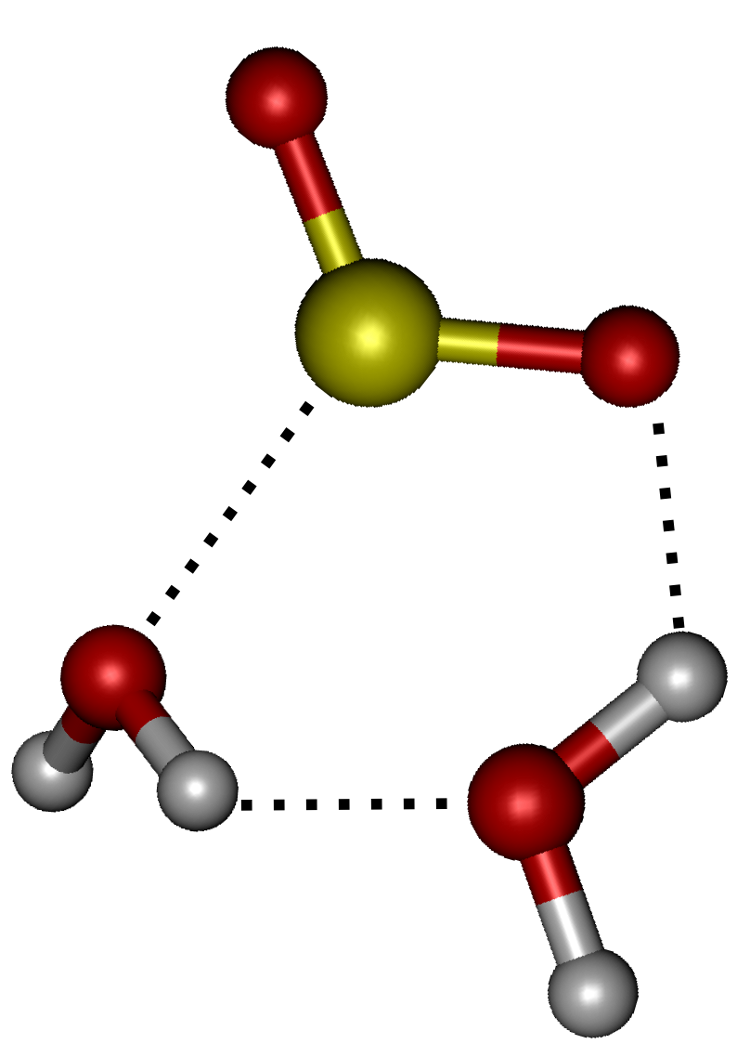
\includegraphics[scale=1.0]{double-cycle-type2-small.png}
		\caption{During the course of MD, the covalent and intermolecular bonds between a \suldiox~and the hydrating waters may form into a ring, resulting in a cyclic hydrate structure. Depicted here is one example of such a cyclic structure, formed by the covalent SO and OH bonds of the two molecule types, the intermolecular hydrogen bonds, and S-O$_{H_2O}$ interactions. The atoms involved are the S (yellow), O (red), and H (white).}
		\label{fig:cyclic-example}
	\end{center}
\end{figure}

\subsection {Graph Theoretical Details}

As noted above, the optimized geometry of the gas phase \suldiox~hydrates suggests cyclic bonding structures. Geometry optimization shows the formation of these cyclic hydrate structures with two or three waters. A different story entirely has the potential to emerge when \suldiox~is placed in a dynamic environment such as in the course of MD simulations of an aqueous surface. Do the cyclic structures also form in the course of a dynamic bonding process on a simulated water surface, where extended hydrating structures influence \suldiox~and water behavior? To study the formation and behavior of cyclic hydrate structures we employ graph theoretical techniques on MD trajectory data. Previous use of graphs in molecular computations were applied to finding stable arrangements of water clusters, ice, hydrogen bonding, extracting topological molecular properties, enumerating complex reaction pathways, and cyclic structure studies.\cite{Anick2002, Huber2007, Radhakrishnan1991, Shi2005, Garcia2004, McDonald1998, Sinanogly1975}

Here we briefly introduce graph theoretical concepts. They have been described well by others with varied application to cyclic structures.\cite{Tutte1984, Balakrishnan2000, Harary1973, Huber2007, Garcia2004, Dury2001} A graph consists of nodes, and edges that connect the nodes. A molecule can be represented with atoms as nodes, and edges for each intramolecular covalent bond connecting the atoms. The set of edges is then further expanded to include intermolecular interactions such as hydrogen bonds and other bonding interactions. Edges may be assigned weights (i.e. bond lengths), types, and can be directional, i.e. pointing from a source node towards a target node. A molecular system including all atoms, bonds, and interactions is thus fully described by a graph. 

To detect cyclic structures in a graph a depth-first or breadth-first search (DFS and BFS, respectively) may be used.\cite{Knuth1997, Cormen 2001} A graph search is a recursive algorithm of queueing nodes and all neighboring nodes while performing a specified procedure on each visited node. This is easily performed on adjacency list or connectivity matrix data structures, iterating through nodes (i.e. atoms) of interest in the graph as starting points of the search. In graph search terminology, all nodes are colored during graph traversal to distinguish unvisited nodes (white), queued nodes (gray), and visited nodes (black). Performing a BFS on a graph, cyclic structures are detected any time a ``gray target'' is encountered when queueing adjacent neighbors of a node. A benefit of BFS is the ability to determine the smallest cyclic structure containing a given node. In the case of \suldiox~hydrate structures, beginning the BFS with the \suldiox-sulfur as the starting, or root node for the search, will discover cyclic bonding structures in order of size. Here we are only concerned with the smallest cyclic structure involving those waters in the first and second hydration shells around the \suldiox. Furthermore, it is possible to reconstruct a cycle's structure by finding its size (number of contributing atoms), and the number of unique waters in the cycle. This allows us to distinguish between various types of cyclic structures encountered.

Several arrangements of cyclic bonding structures are shown in Figure \ref{fig:cyclic-structures} for a \suldiox~molecule with three waters. Cycles with fewer or greater numbers of waters are also possible and encountered during MD. Cycle types \Rmnum{1}, \Rmnum{2}, \Rmnum{3} in Figure \ref{fig:cyclic-structures} are cyclic structures in which the \suldiox~is a member of the cycle. Types \Rmnum{4} and \Rmnum{5} do not involve the \suldiox~in the bonding cycle, but are commonly encountered as the smallest cycle types formed near the \suldiox. Type \Rmnum{3} is of particular interest because the \suldiox~in this cycle has the most frequently occurring bonding coordination (``SO'', as shown later).

\begin{figure}[h!]
	\begin{center}
		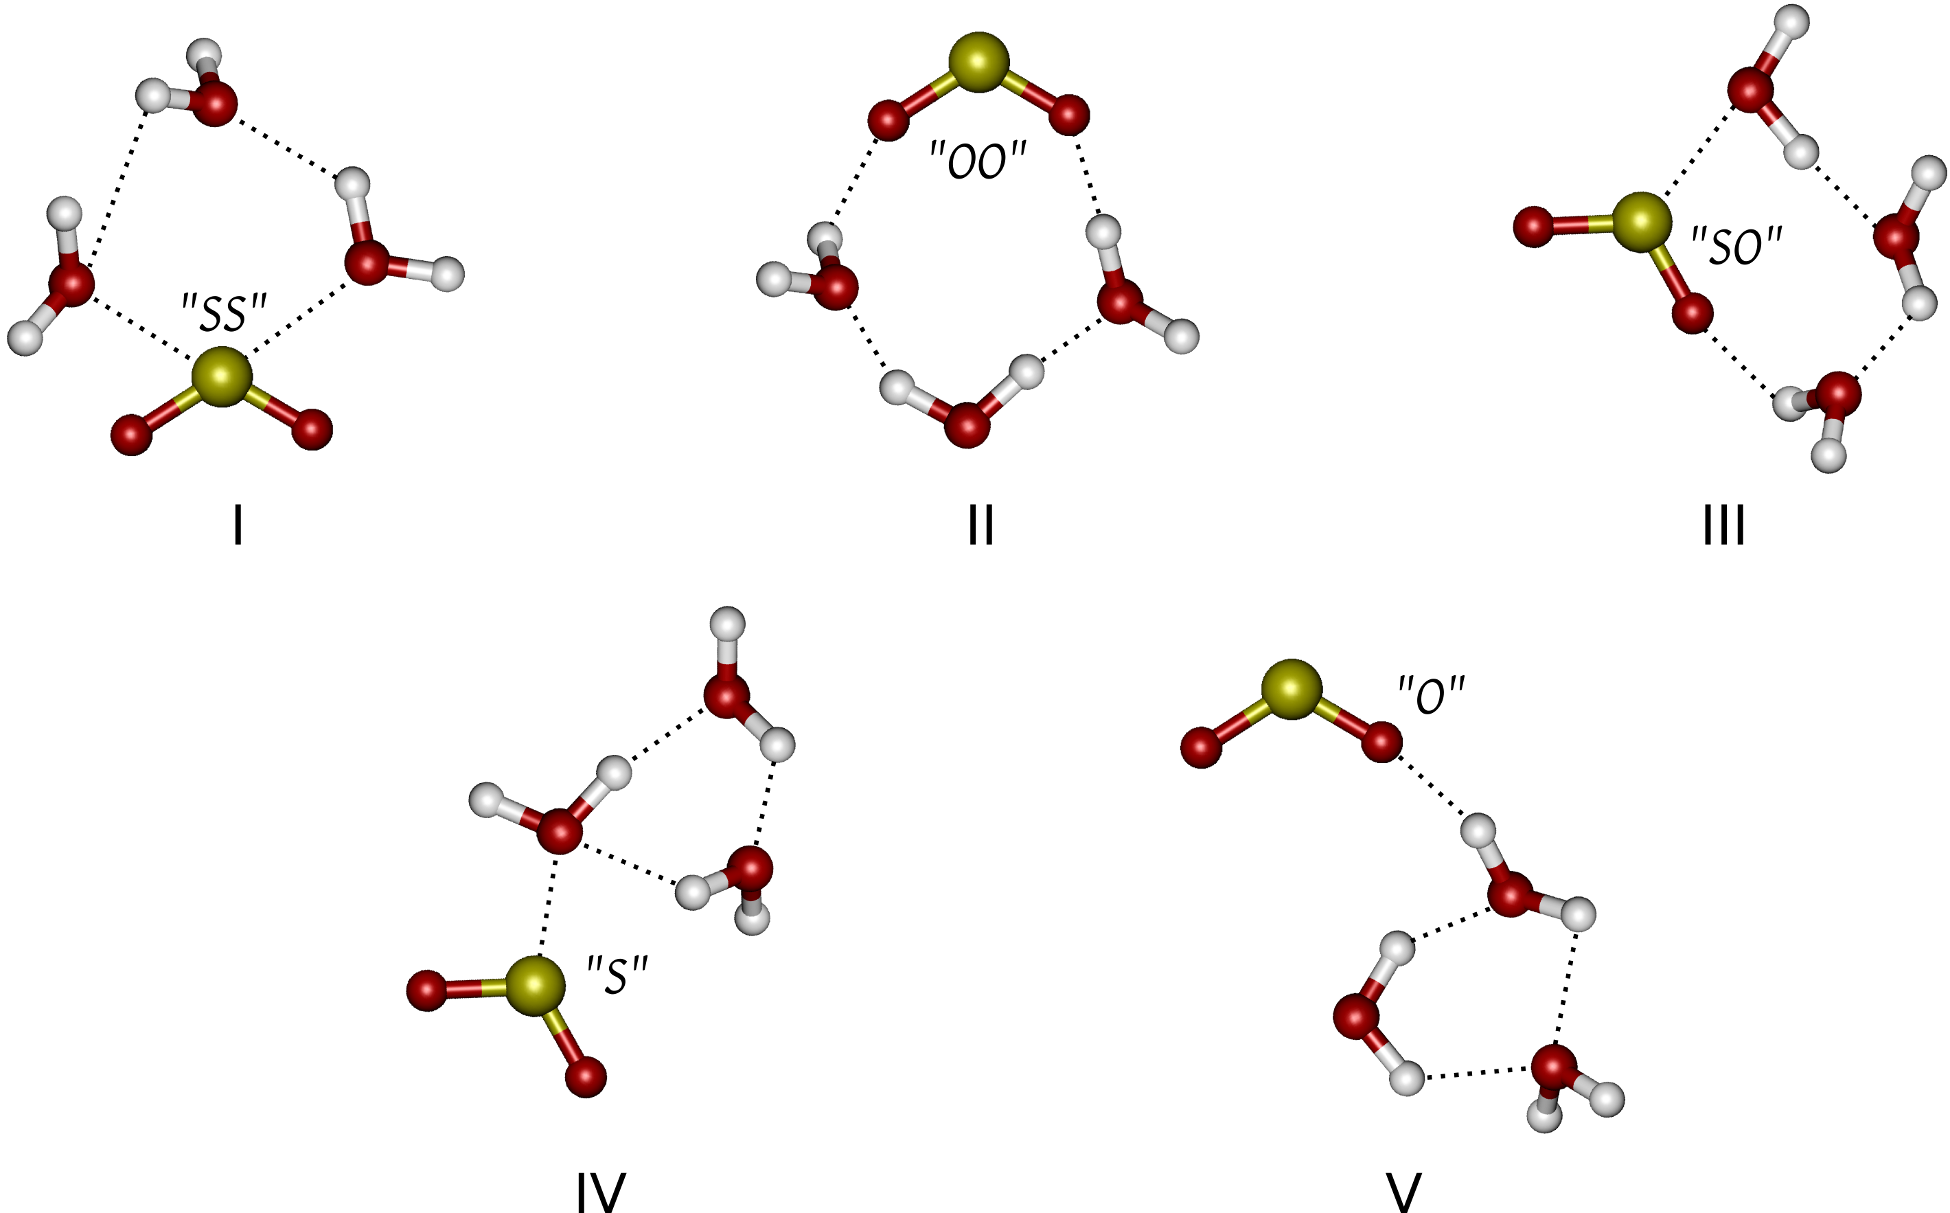
\includegraphics[scale=1.0]{cycle-types-small.png}
		\caption{\suldiox~in various cyclic structures encountered during MD simulations with water. The cartoons show the five types of cyclic structures, numbered for reference. The cyclic structures may involve any number of waters, but here each structure is shown with three waters. Type \Rmnum{3} is formed by a \suldiox~with the ``SO'' bonding coordination, which is the most dominant bonding coordination encountered. Each hydrate structure is labelled with its corresponding bonding coordination type using the nomenclature described in the text.}
		\label{fig:cyclic-structures}
	\end{center}
\end{figure}

Baer et al. presented a detailed geometric and spectroscopic breakdown of type \Rmnum{3} cycles with two and three waters from their DFT calculations.\cite{Baer2010} Given the information of the number of waters, atoms, and bonds involved in the bonding cycles, we find that of the three-water type \Rmnum{3} cycles, there exist two structural varieties, shown in Figure \ref{fig:type-3-varieties}, that differ in the set of water atoms involved in the cyclic structure. Type \Rmnum{3}-A (shown in Figure \ref{fig:type-3-varieties}A) is arranged with each water contributing an OH bond to the structure of the cycle. Type \Rmnum{3}-B involves a single water contributing an OH, whereas the other two waters contribute only the oxygen atom or the entire water molecule to the structure, respectively. This nuance of the type \Rmnum{3} structures involving three waters, and the overall distribution of structures are presented in more detail later. We also show the distribution of cyclic structures encountered during MD simulations to further understand the behaviors of \suldiox-hydrates at the water surface.

\begin{figure}[h!]
	\begin{center}
		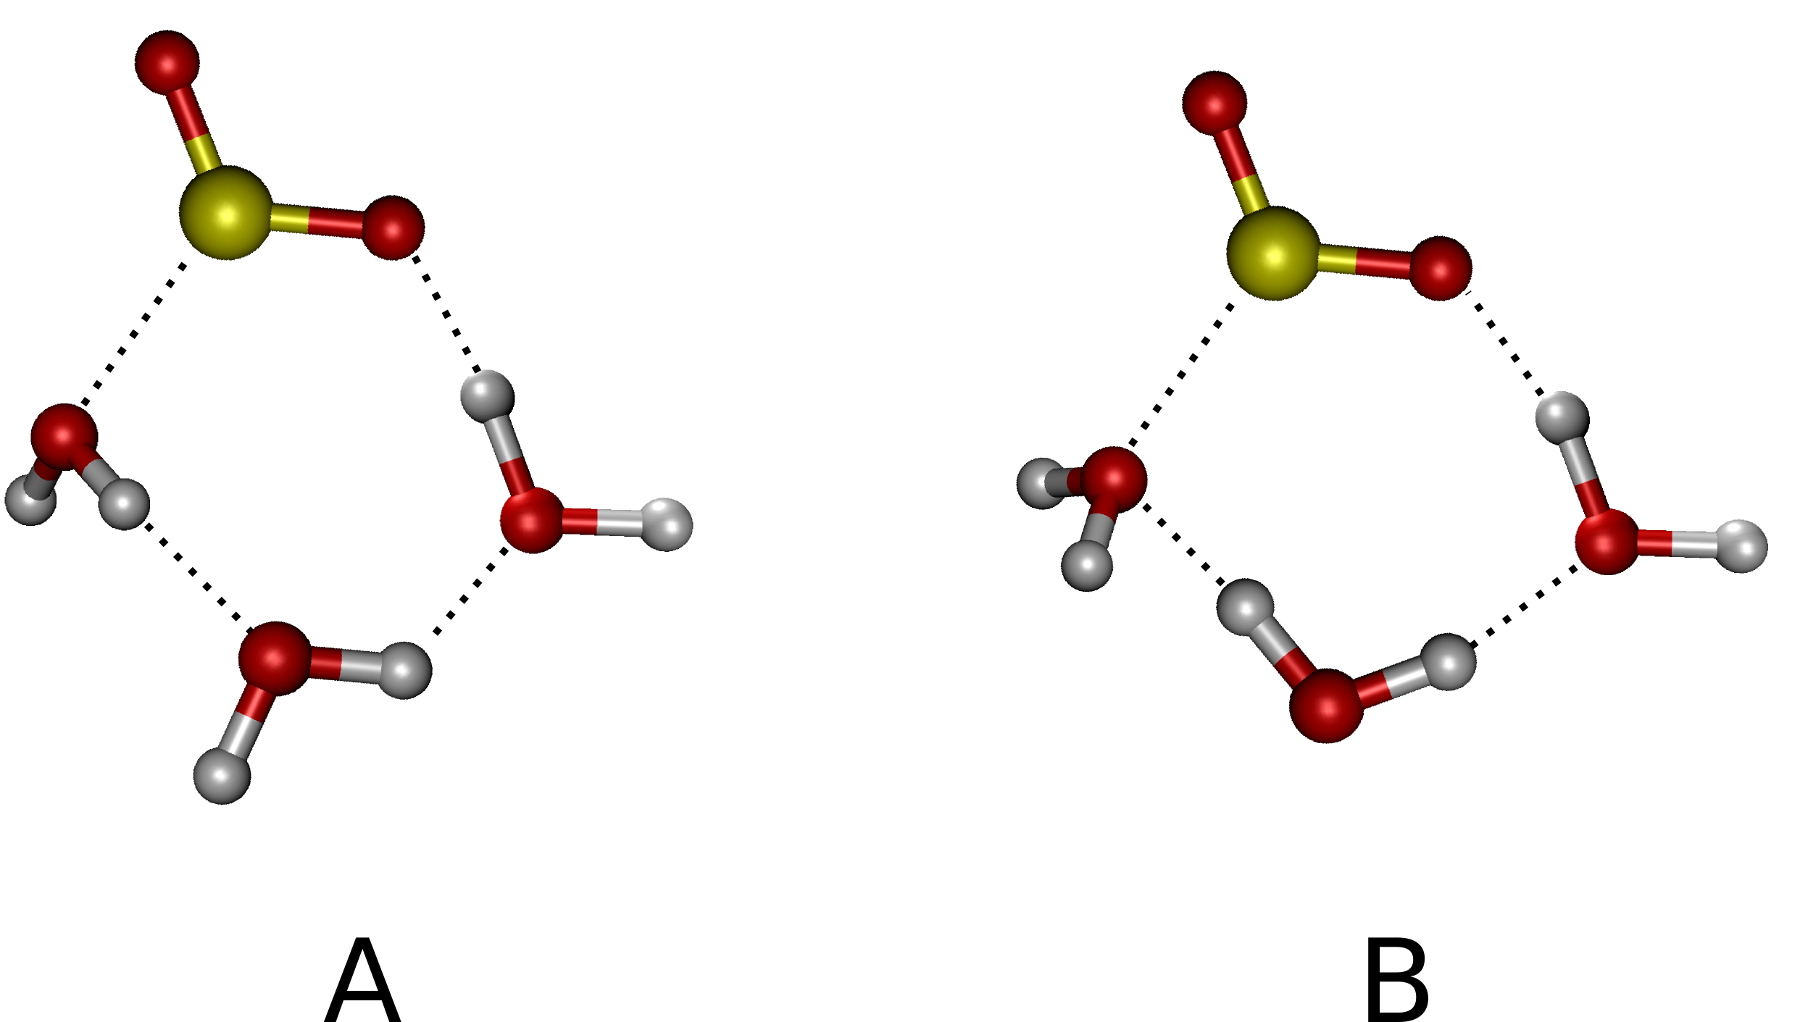
\includegraphics[scale=1.0]{triple-cycle-types-small.png}
		\caption{Type \Rmnum{3} cyclic structures (see Figure \ref{fig:cyclic-structures}) are found to occur in two varieties that are distinguished by the water atoms contributing to the cyclic structure. In ``type A'' the cycle is formed by an OH bond contributed by each water, and the SO bond of the \suldiox. ``Type B'' involves an oxygen atom from one water, an OH bond from a second water, and all atoms of the third water.}
		\label{fig:type-3-varieties}
	\end{center}
\end{figure}


%comp methods
\section{Computational Methods}

On-the-fly ab initio molecular dynamics simulations were performed with the QUICKSTEP package (Car-Parrinello method of MD), which is an implementation of the Gaussian plane wave method using the Kohn-Sham formulation of density functional theory (DFT).\cite{VandeVondele2005} The Kohn-Sham orbitals are expanded using a linear combination of atom-centered Gaussian-type orbital functions. The electronic charge density was described using an auxiliary basis set of plane waves. Energies and forces from on-the-fly simulation sampling of the Born-Oppenheimer surface were calculated for each MD step using the Gaussian TZV2P basis set with a cutoff of 280 Ry, the exchange-correlation functional of Becke, Lee, Yang, and Parr (B3LYP),\cite{LEE1988} and the atomic pseudo-potentials of the Goedecker, Teter, and Hutter type.\cite{Goedecker1996} A simulation timestep of 0.5 fs was used, with a Nos\'{e}-Hoover thermostat set at 210K and 300K for the ``cold'' and ``hot'' simulations, respectively, using a coupling constant of 1000 fs. %These computational parameters were verified to yield a reasonable description of bulk room temperature water when simulating a neat-water system. 

Initially, 20 equilibrated boxes of side-lengths 8.9545\angs, with 24 randomly packed water molecules were used. Ten of the boxes were used for each of the cold and hot simulations. A sulfur dioxide molecule was randomly placed onto the surface within 2.5\angs~of a water molecule centrally located above the waters in the z-axis. A copy of the initial system cubes were then expanded along one axis (z-axis) to 30\angs. The system energy was minimized through a geometry optimization. Subsequently, the system was equilibrated for 1 ps in canonical ensemble (NVT) conditions. Periodic boundaries were set on the two short axes to form an infinite slab. The equilibrated systems were then simulated for a further 20 ps in the microcanonical ensemble (NVE), with trajectory snapshots recorded every 0.5 fs. The initial 1 ps equilibration trajectory was not included in the final analysis. This simulation process resulted in 40,000 time steps of system trajectory for analysis in each of the hot and cold replicas of the system, for a total of 400,000 timesteps at each temperature.

% coordination results
\section {Sulfur Dioxide Bonding Coordinations}

The bonding coordination of each \suldiox~was determined at each timestep of the simulations. Figure \ref{fig:bonding-coordinations} shows the distribution of bonding coordinations of the surface \suldiox, as a percentage of all bonding coordinations encountered for both the cold (blue) and hot (red) trajectories. A first visual inspection reveals several trends. At both temperatures the \suldiox~spends much of the time unbound without any bonding to the surface waters. The cluster of the three most populated coordinations is comprised of the ``S'', ``SO'', and ``SOO'' bonding types. This grouping represents the coordinations with a single bond through the sulfur, and up to two interactions through the \suldiox-oxygens. In this coordination group the ``SO'' is the most populous, but in no way dominates the bonding types as the difference in populations is less than 2\% and 5\% within the cold and hot simulations, respectively. The second and third most populated bonding coordinations (excluding the unbound state) are the ``S'' and ``SOO'', however their distributions differ between temperatures. In cold simulations the ``S'' and ``SOO'' coordinations occur nearly equally (18.8\% and 18.1\%, respectively). The hotter temperature simulation shifts the distribution such that the ``S'' occurs 4.6\% less frequently than in the cold, and the ``SOO'' occurs 8.6\% less often. The distribution of bonded coordinations (those excluding the ``unbound'' state) in the hot temperature has a clear first and second most frequent coordination: ``SO'' and ``S'', respectively. 

\begin{figure}[h!]
	\begin{center}
		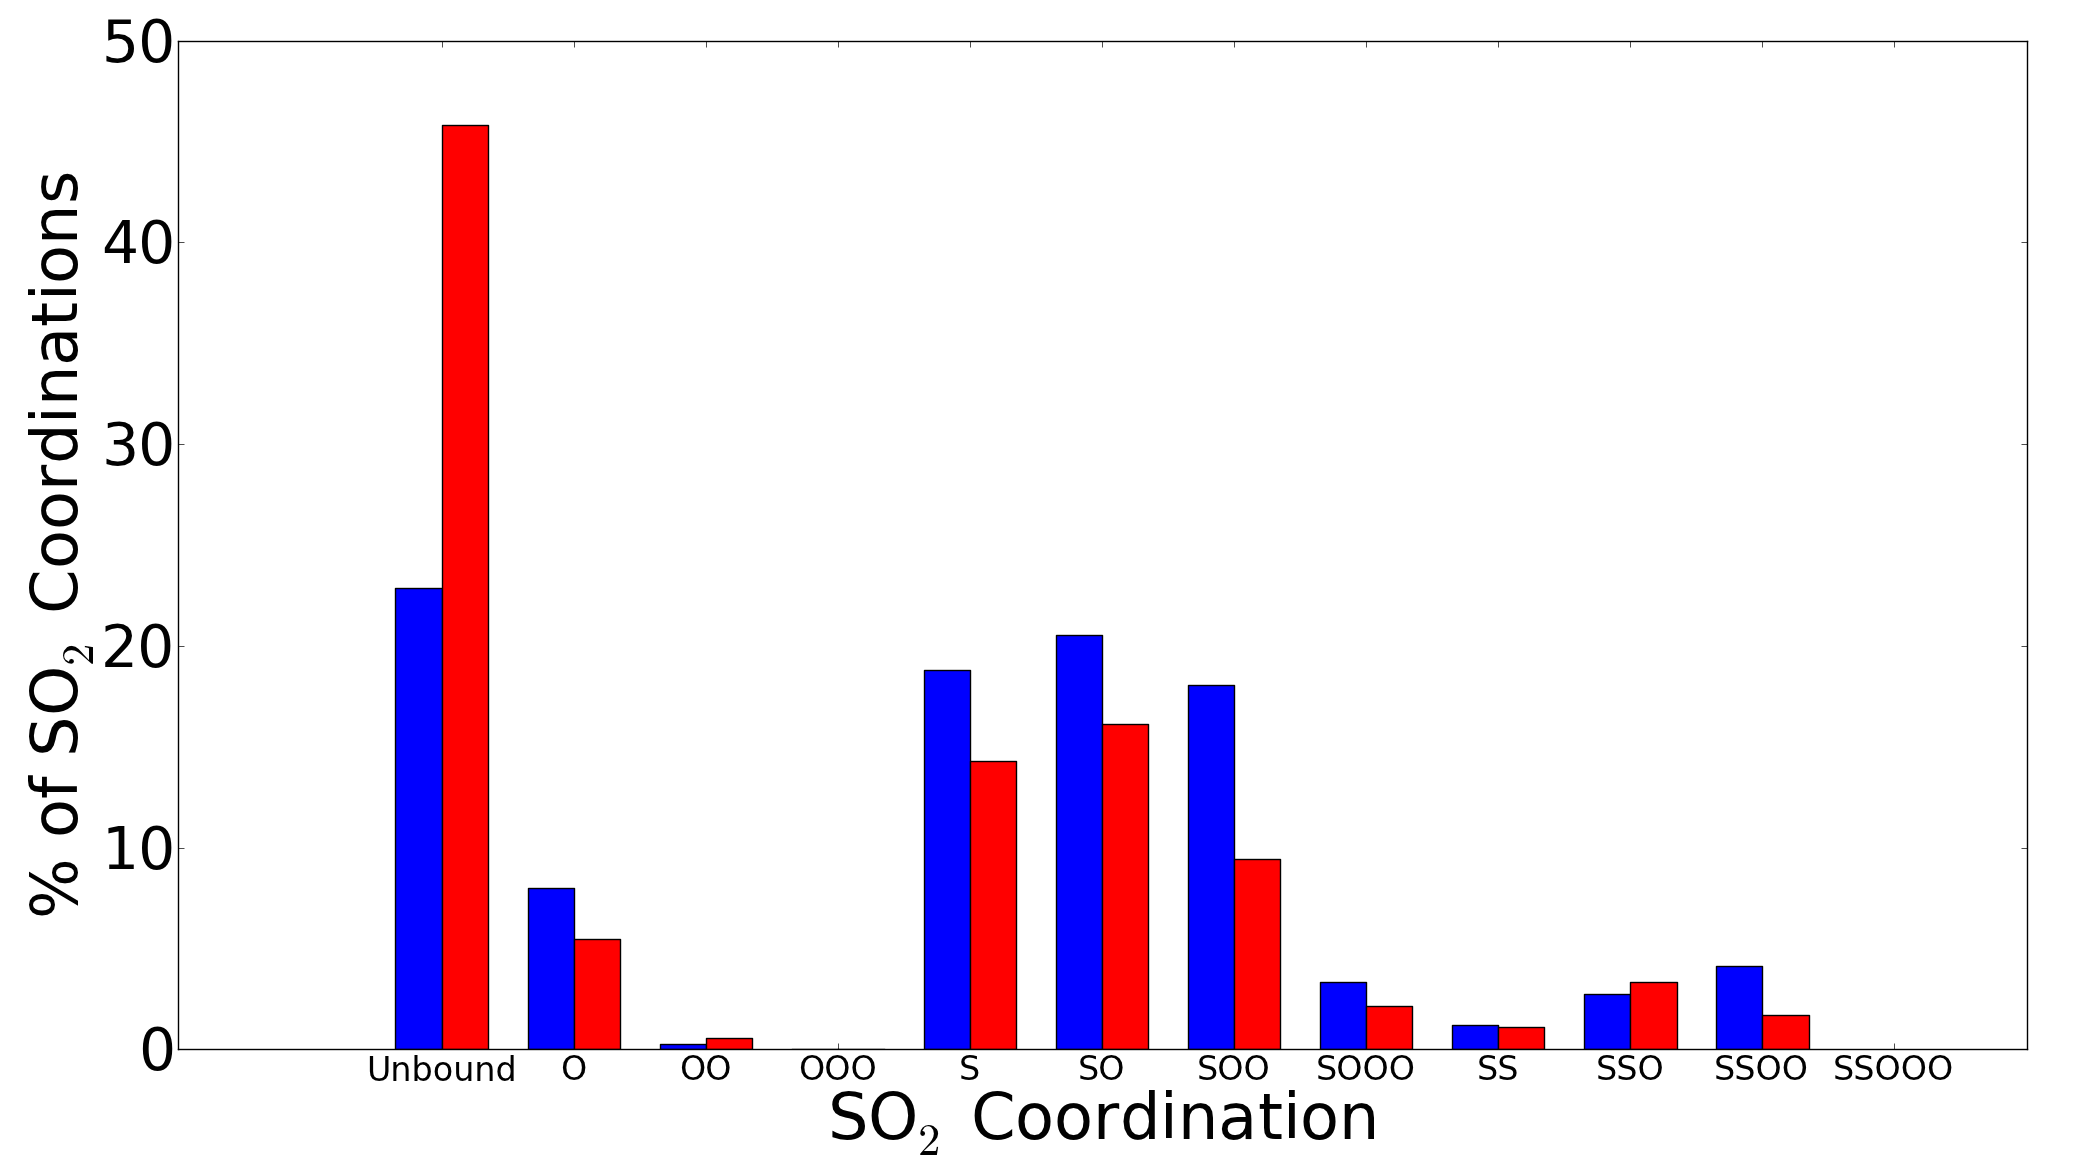
\includegraphics[scale=1.0]{coordination-distributions.png}
		\caption{The \suldiox~bonding coordinations occur with different frequencies at the surface under hot and cold temperature conditions. Shown above is the distribution of bonding coordinations of the cold (blue) and hot (red) \suldiox~over the entire set of trajectories. The values are the percentage of MD timesteps spent in the given bonding coordination.}
		\label{fig:bonding-coordinations}
	\end{center}
\end{figure}

	Several conclusions about the bonding behavior of \suldiox~to surface waters stem from this distribution of coordinations. Clearly the hot \suldiox~spends more time than the cold \suldiox, 45.8\% versus 22.8\%, respectively, completely unbound from the surface waters. This does not necessarily imply a complete desorption into the gas phase, but likely only a brief sojourn away from the surface waters, with all interactions and bond lengths longer than the cutoff criteria used for the analysis. The unbound coordination data is also supported by our recent spectroscopic experiments that resulted in increased \suldiox~surface binding at colder temperatures.\cite{Ota2011} Furthermore, the most frequently occurring bonding coordinations are ``S'',``SO'', and ``SOO'', with ``SO'' being the most populated at both temperatures. Baer et al. also concluded that these three coordinations were the most frequent for a room temperature simulation, and specifically identified the ``SO'' and ``SOO'' as most common in their study.\cite{Baer2010}

	Looking closer at the coordination types it is notable that coordinations lacking any sulfur interactions (e.g. ``O'', ``OO'', etc.) form infrequently (approximately 6\% and 8\% of the total hot and cold bonding coordinations, respectively). A bonding coordination with at least a single sulfur interaction is clearly favored over \suldiox~``oxygen-only'' bonding to waters. In our previous classical simulations of \suldiox~on water we concluded that during adsorption and throughout the interface, the \suldiox~orients so that its sulfur tends to the \wat~bulk side of the interface.\cite{Shamay2011} The coordination distributions here support the idea that binding through the sulfur is preferable, to the extent that a non-sulfur coordination is not often formed during the course of all our simulations.

% Baer's assymetric oxygen binding
Baer et al. performed this coordination analysis for their single-temperature study, but discriminated between \suldiox~binding through the two different oxygens. They concluded that there is asymmetric hydrogen bonding through the \suldiox-oxygens, with one oxygen binding more often than the other. This is supported by the findings here where the double oxygen coordinations (e.g. ``OO'', ``SOO'', etc.) represent a lower percentage of the coordinations than the single oxygen counterparts (e.g. ``O'', ``SO'', etc.). Furthermore, a triple-oxygen coordination (e.g. ``OOO'', ``SOOO'', etc.) is very rarely encountered. Three \suldiox-oxygen bonds only form if both \suldiox-oxygens are interacting with water hydrogens. Our finding that triple-oxygen coordinations rarely form, and that double-oxygen coordination are less frequent than the single-oxygen counterparts, complements Baer et al's conclusion about the asymmetry in the oxygen interactions.

Having established the preference for an interaction through the \suldiox-sulfur atom, we look to the right side of Figure \ref{fig:bonding-coordinations} at the double-sulfur coordinations (e.g. ``SS'', ``SSO'', ``SSOO'', etc.). From the data it is clear that single-sulfur coordinations are overwhelmingly preferred over double-sulfur ones. Adding a third oxygen atom is also unfavorable as the ``OOO'', ``SOOO'', and ``SSOOO'' combined represent less than 4\% of the trajectories, and the comparison between ``SOO'' to ``SOOO'' shows a very large decrease in occurrences.

A picture can now be formed of a typical \suldiox~molecule adsorbed to a water surface across both temperatures in this study. Often the \suldiox~will remain unbound from the interface, more than twice as often when the temperature is hot. The \suldiox~will form at least one interaction with neighboring waters through the sulfur, and will then bond asymmetrically through one of the oxygens either once or twice to water hydrogens. The \suldiox-oxygen bonds will form and break repeatedly throughout a trajectory, and overall the most dominant bonding coordination will be the ``SO'' bonding arrangement.

\subsection {Temperature Effects on Bonding Coordinations}

The binding behavior of the \suldiox~is altered by changing the temperature of the system, as evidenced in the shift in bonding coordination populations of Figure \ref{fig:bonding-coordinations} from cold to hot. In the cold temperature, the bound coordinations are overall more populated than when hot. Conversely, the hot temperature system is much more often unbound (nearly half of the simulated time) than when the temperature is cold. A decrease in temperature causes a clear change to the surface binding behavior of \suldiox. At colder temperatures a \suldiox~molecule will bind more strongly to a water surface than at higher temperatures.

%On the cold water surface, the ``S'' and ``SO'' are more populated than for the hot system. The relative decrease of these coordinations are matched in the hot surface by an increase of the ``SOO'' configuration. This speaks to a dramatic difference in the surface behavior of \suldiox~at the two temperatures. The cold \suldiox~spends nearly equal time in the ``S'' and ``SOO'' coordinations, but nearly 20\% more time in the ``SO''. Thus, the addition or removal of a bond through the \suldiox-oxygen to a neighboring coordination (e.g. addition of an oxygen bond from ``SO'' to ``SOO'', or removal of the bond from ``SO'' to ``S'') is equally probable, as long as the sulfur interaction with the water oxygen does not break. 

Figure \ref{fig:rdf} shows the radial distribution functions (RDF) of \suldiox~to water atoms for both cold (blue) and hot (red) temperatures. The S-O$_{H_2O}$ RDFs are overall very similar. A difference between the cold and hot simulations appears in the first peak of both RDFs. The cold RDFs have a slightly taller and narrower first peak than the hot counterpart, and the peak is located at a slightly shorter distance. Along with the slightly larger population of the cold ``S'' and ``SO'' coordinations in the cold surface, the RDF indicates that since bonding occurs frequently through the sulfur, the cold \suldiox-sulfur interacts more closely with the surface water oxygens than in the hot waters. This suggests that the cold \suldiox~favors the more ``sulfur-centric'' bonding coordinations (e.g. ``S'', ``SO'', ``SOO''). The broader first peak of the hot RDFs likely indicates that the sulfur atoms have a slightly larger array of bonding environments to water oxygens. Similarly, the \suldiox-oxygen displays the same difference in the first peak on the left plot of Figure \ref{fig:rdf}. 

\begin{figure}[h!]
	\begin{center}
		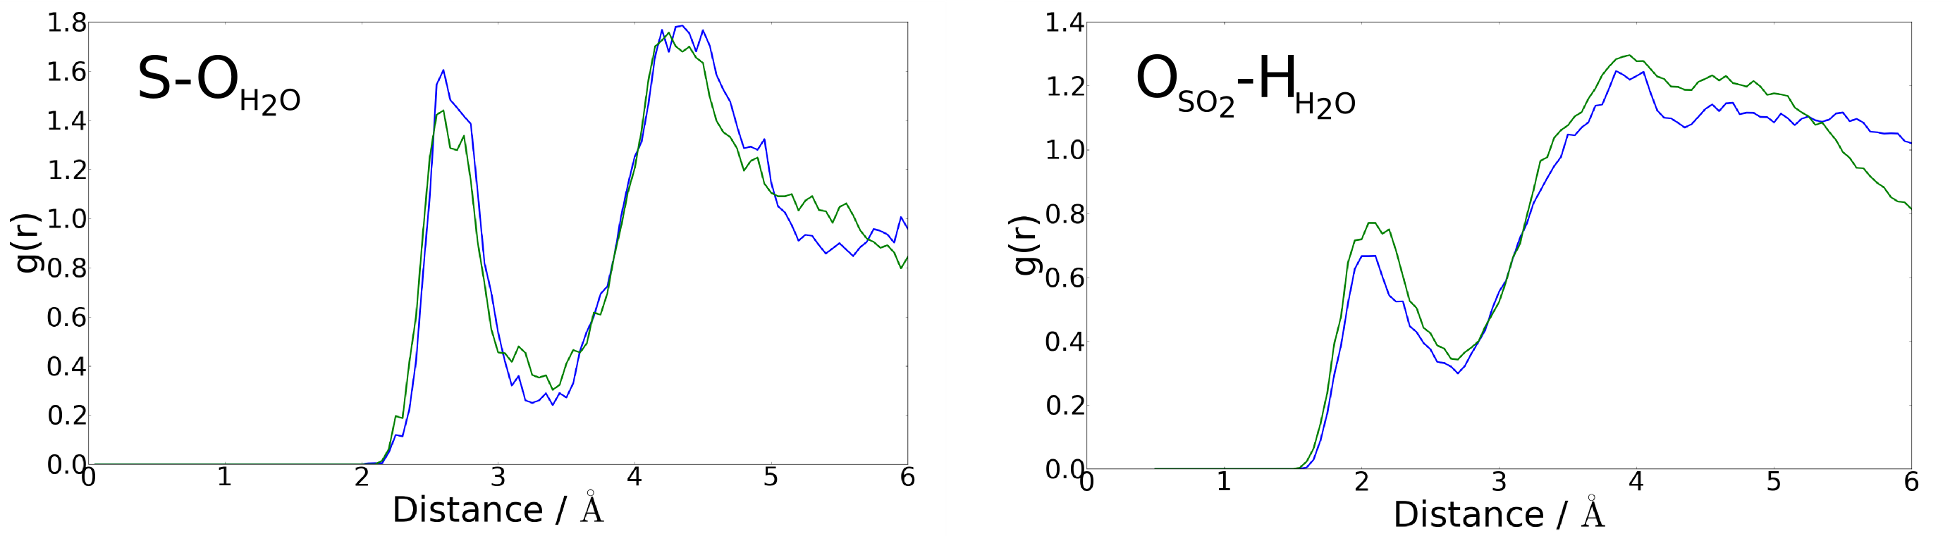
\includegraphics[scale=1.0]{rdf-small.png}
		\caption{Radial distribution functions (RDF) show the subtle change in how the hydrating waters around \suldiox~reposition as the temperature is increased from cold (blue) to hot (red). Shown are the two correlations between sulfur and water oxygens (right) and the \suldiox-oxygen and water hydrogens (left).}
		\label{fig:rdf}
	\end{center}
\end{figure}

\subsection {Bonding Transitions}

During the course of each simulation, the \suldiox~bonding coordination was determined and recorded for each timestep. From the coordination data we extract not only the populations of the various bonding coordinations, but also the frequencies of transitions between the different coordinations (i.e. the number of times each \suldiox~switched from one coordination type to another). With this data we have generated the directed graphs of Figure \ref{fig:coordination-transitions} depicting the cold and hot (Figure \ref{fig:coordination-transitions} left and right, respectively) bonding coordinations as circular colored nodes.\cite{Ellson2004,Gansner1999} The transitions between the coordinations are depicted as directed edges pointing in the direction of the transition from one bonding coordination to another. The populations of the coordinations are depicted by both the node size and coloration (larger and darker red coordinations occur more frequently). Populations of the transitions between coordinations are depicted by arrow thickness, with thicker lines corresponding to more frequent transitions. Additionally, the transition lines are numbered to the right of each line with the number of times each transition occurred. 

\begin{figure}[h!]
	\begin{center}
		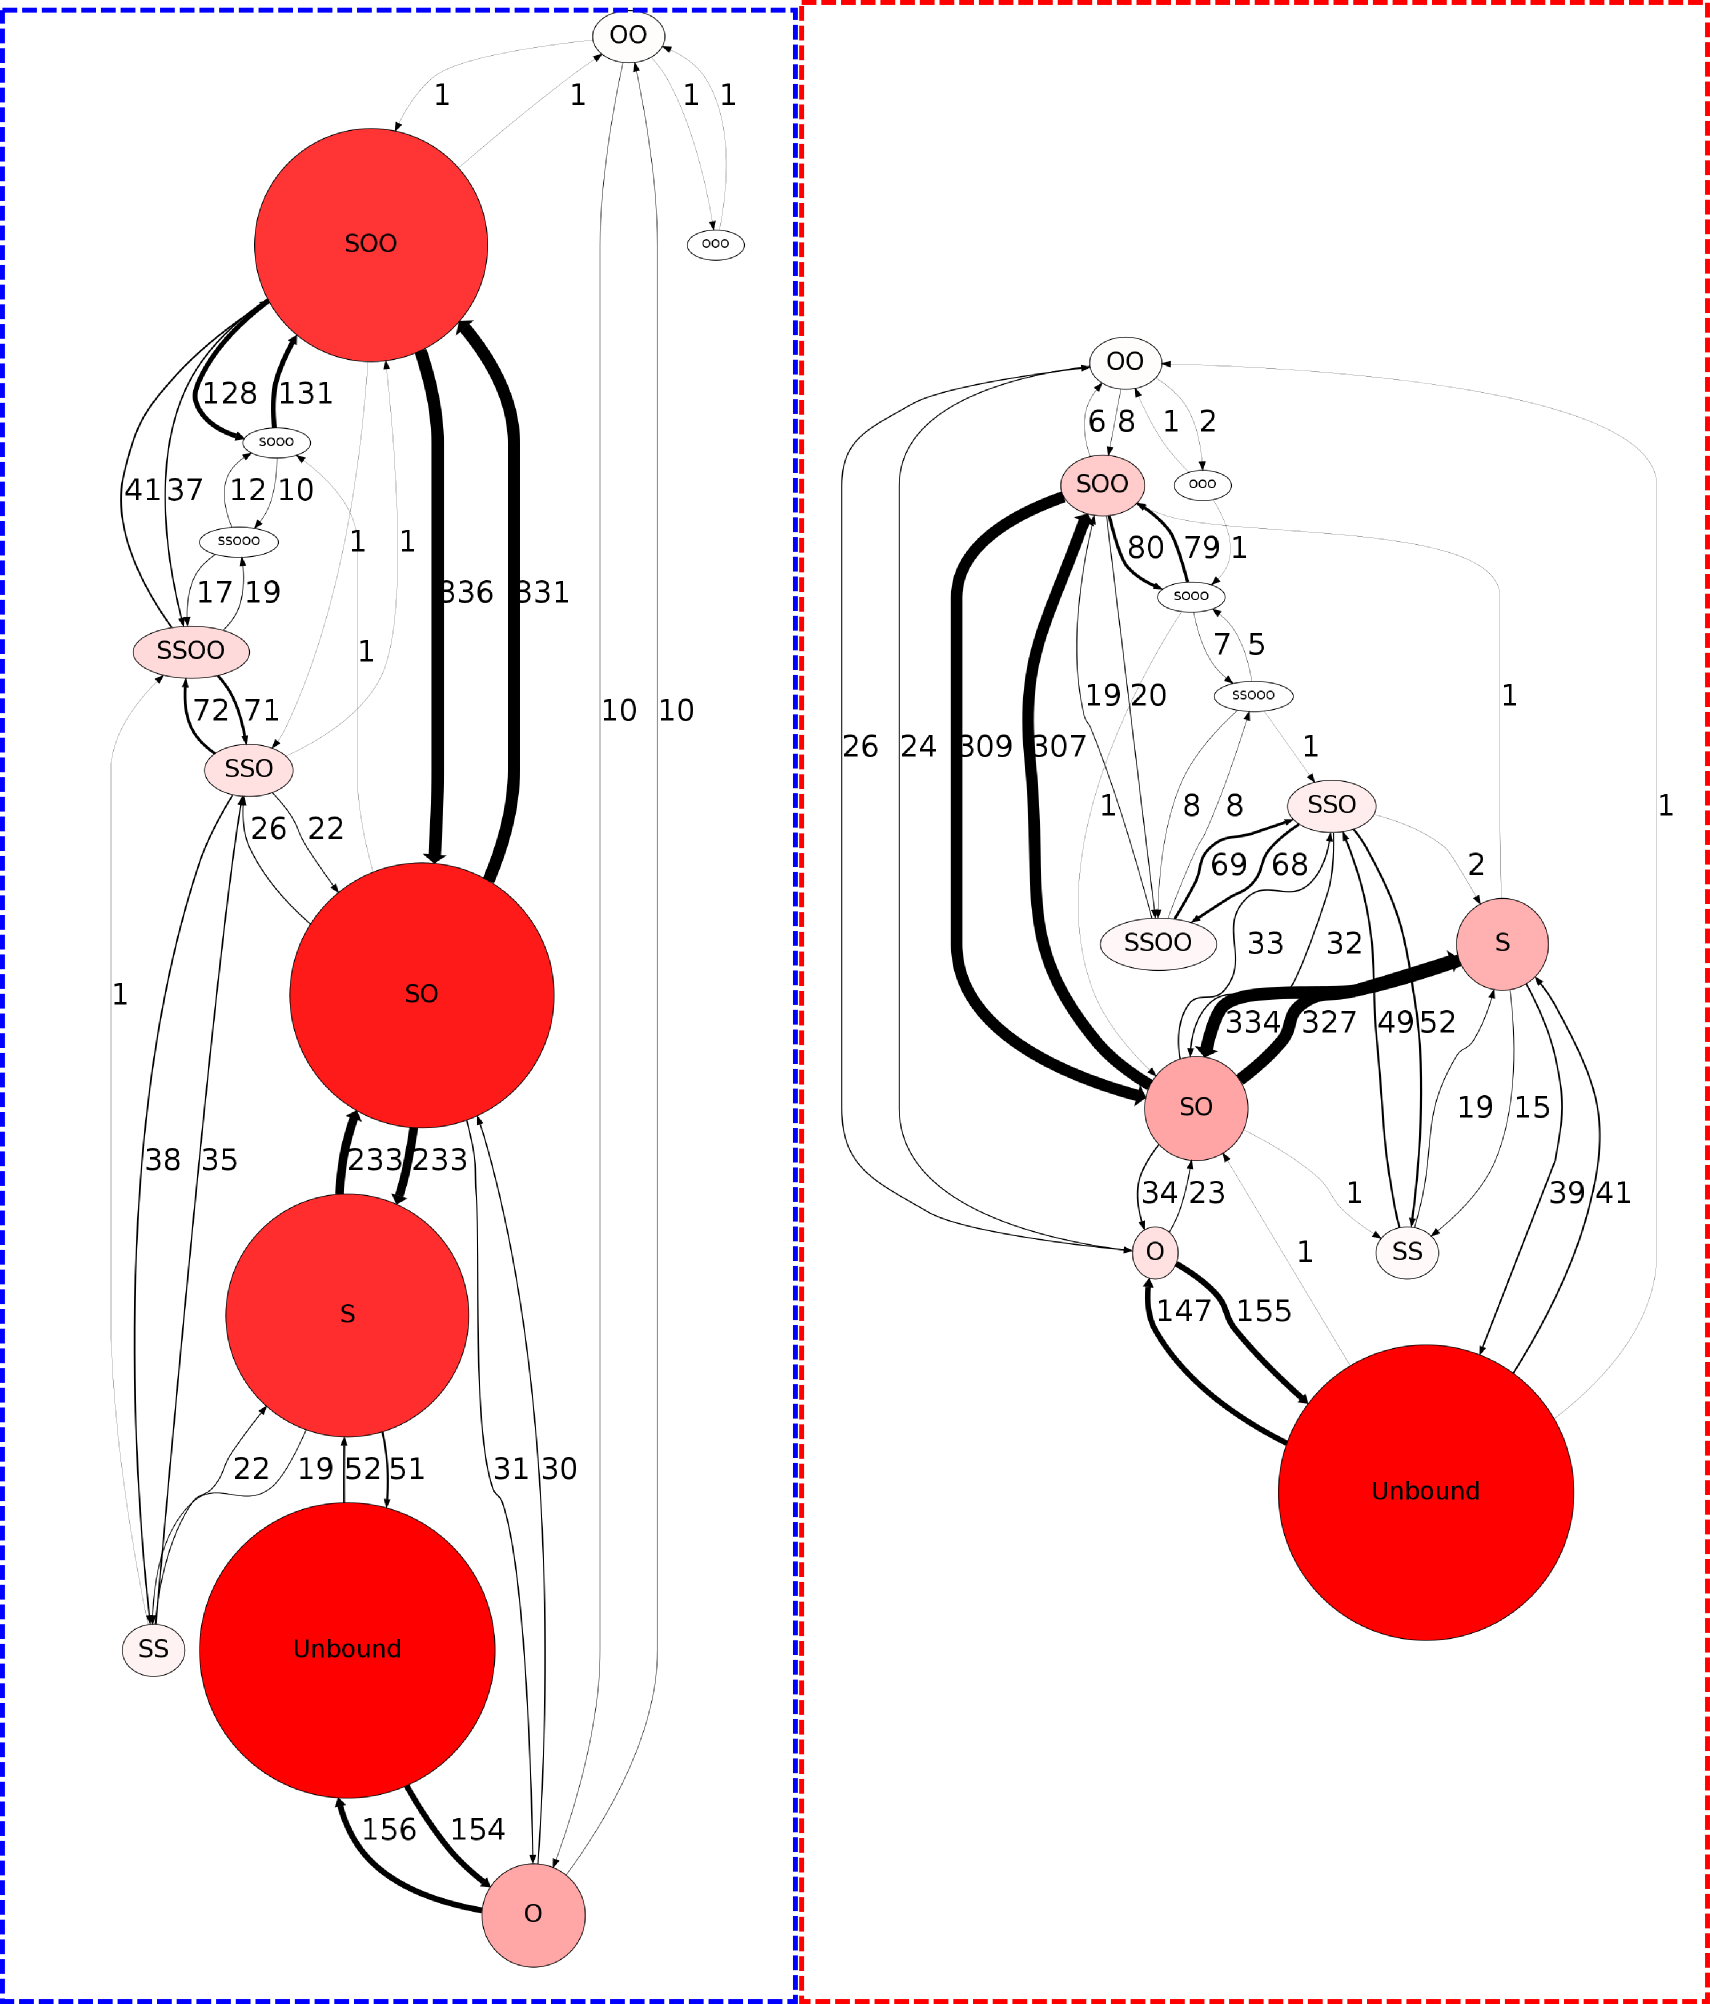
\includegraphics[scale=1.0]{coordination-transitions.png}
		\caption{The bonding coordinations of \suldiox~on a water surface rapidly change as bonds break and form throughout the MD trajectories. Depicted here is a graph of the bonding coordinations, shown as colored nodes of varying size. Larger and more darkly colored coordination nodes are those more often encountered during MD (see Figure \ref{fig:bonding-coordinations}). The directed edges between the nodes represent the number of times the coordination transition occurred. Thicker lines correspond to a greater number of transitions between coordinations. The number of times a given transition occurred is labelled to the right of the corresponding line.}
		\label{fig:coordination-transitions}
	\end{center}
\end{figure}

As expected for the more populated coordinations, there are generally more transitions between larger nodes in Figure \ref{fig:coordination-transitions} than transitions to less populated coordinations. Insights to the bonding process are made clearer from these graphs. In the cold system graph of Figure \ref{fig:coordination-transitions}, we find that the majority of transitions are between the unbound and ``O'' nodes, and between the single-sulfur coordinations (e.g. ``S-SO'', ``SO-SOO'', etc.) The number of transitions within these groups of bonding coordinations is an order of magnitude larger than any other transition. This indicates that while the \suldiox~is bound in any of the most populated bonding coordinations, it is actively binding and unbinding the oxygens to form the other coordinations, typically those with a single sulfur interaction. Clearly, the \suldiox-sulfur bond to water oxygens is stronger than its oxygen bonds to water-hydrogens. The \suldiox-oxygens are actively and constantly forming and breaking bonds to neighboring waters. In the graph of the hot system in Figure \ref{fig:coordination-transitions} (right), the transition frequencies follow the same trend as in the cold system, increasing with adjacent node size. %One very surprising result is in the transition from ``SOO-SOOO''. This transition frequency does not follow from the adjacent node sizes, as the ``SOOO'' node represents less than 5\% of the bonding coordinations. This is indicative of a very rapid cycle of forming and breaking of bonds to the second \suldiox-oxygen. As noted earlier, it is likely that ``SOO'' coordinated \suldiox, asymmetrically binding twice through a single oxygen, is being pulled further into the water interface. It is likely more surrounded by waters, and in the hot system it can more easily form a brief third hydrogen bond to a water through the second \suldiox-oxygen. Because the triple-oxygen coordination is not as favorable, it quickly breaks the bond and the \suldiox~returns to the ``SOO'' coordination.

Given the information we have about the frequencies of bonding coordination transitions, it is possible to draw a likely route of adsorption beginning with an unbound \suldiox. From the unbound coordination, the \suldiox~can bind to waters either through the sulfur or an oxygen to enter the ``S'' or ``O'' coordinations, respectively. At both temperatures we find that the coordination transition in Figure \ref{fig:coordination-transitions} from unbound to ``O'' occurs over three times more than the transition from unbound to ``S''. We find two possibilities that may explain this difference. The single H-bonding of the ``O'' coordination may form more easily, but also break quickly after formation, accounting for the higher transition frequency. Otherwise, the ``O'' coordination may be the first step in adsorption of an unbound \suldiox, where a subsequent addition of an \suldiox-sulfur interaction to a water oxygen would lead to a transition to the most frequent coordination, ``SO''. In the latter case, any adsorption of \suldiox~proceeds through an oxygen binding, accounting for the increased unbound-``O'' transition frequency, but because it is likely a less-stable coordination, its population is less than the equivalent ``S'' or ``SO'' configuration.

To verify if the ``O'' coordination forms from, and breaks quickly to the unbound coordination as is suggested by the transition frequency plots in Figure \ref{fig:coordination-transitions}, the lifespans of the various coordinations are plotted in Figure \ref{fig:coordination-lifespans}. Each point in the plot represents a time during the simulation in which the \suldiox~formed the respective coordination. The vertical ``lifespan'' position is calculated directly from the amount of time spent in the given coordination before changing to another. Both cold (blue) and hot (red) data are plotted. The data of Figure \ref{fig:coordination-lifespans} show that most coordination configurations last a very brief time, with the majority forming for under 1 ps. The three most populous coordinations, ``S'', ``SO'', ``SOO'' (as determined from Figure \ref{fig:bonding-coordinations} by percentage) in both temperatures have coordination lifetimes of just over 2 ps, in some instances lasting up to 5-6 ps. The brevity of lifespans overall speaks to the dynamic nature of the \suldiox~surface binding. The length of time in each coordination parallels the populations of the coordinations, and suggests an ordering of steady states among various bonding coordinations. The ``unbound'' configuration stands out as an anomaly amongst the lifespans of the other bonding coordinations. The few lifespans above 3 ps, up to 10 ps long, suggest a \suldiox~that not only unbinds from the water surface, but that it also recedes far enough to avoid a quick rebinding and coordination change to ``S'' or ``O''. Those data points of a few long lived unbound species indicate times when the \suldiox~is far from the water, residing in the gas phase until the necessary water rearrangement occurs and it is drawn back to the surface to rebind.

\begin{figure}[h!]
	\begin{center}
		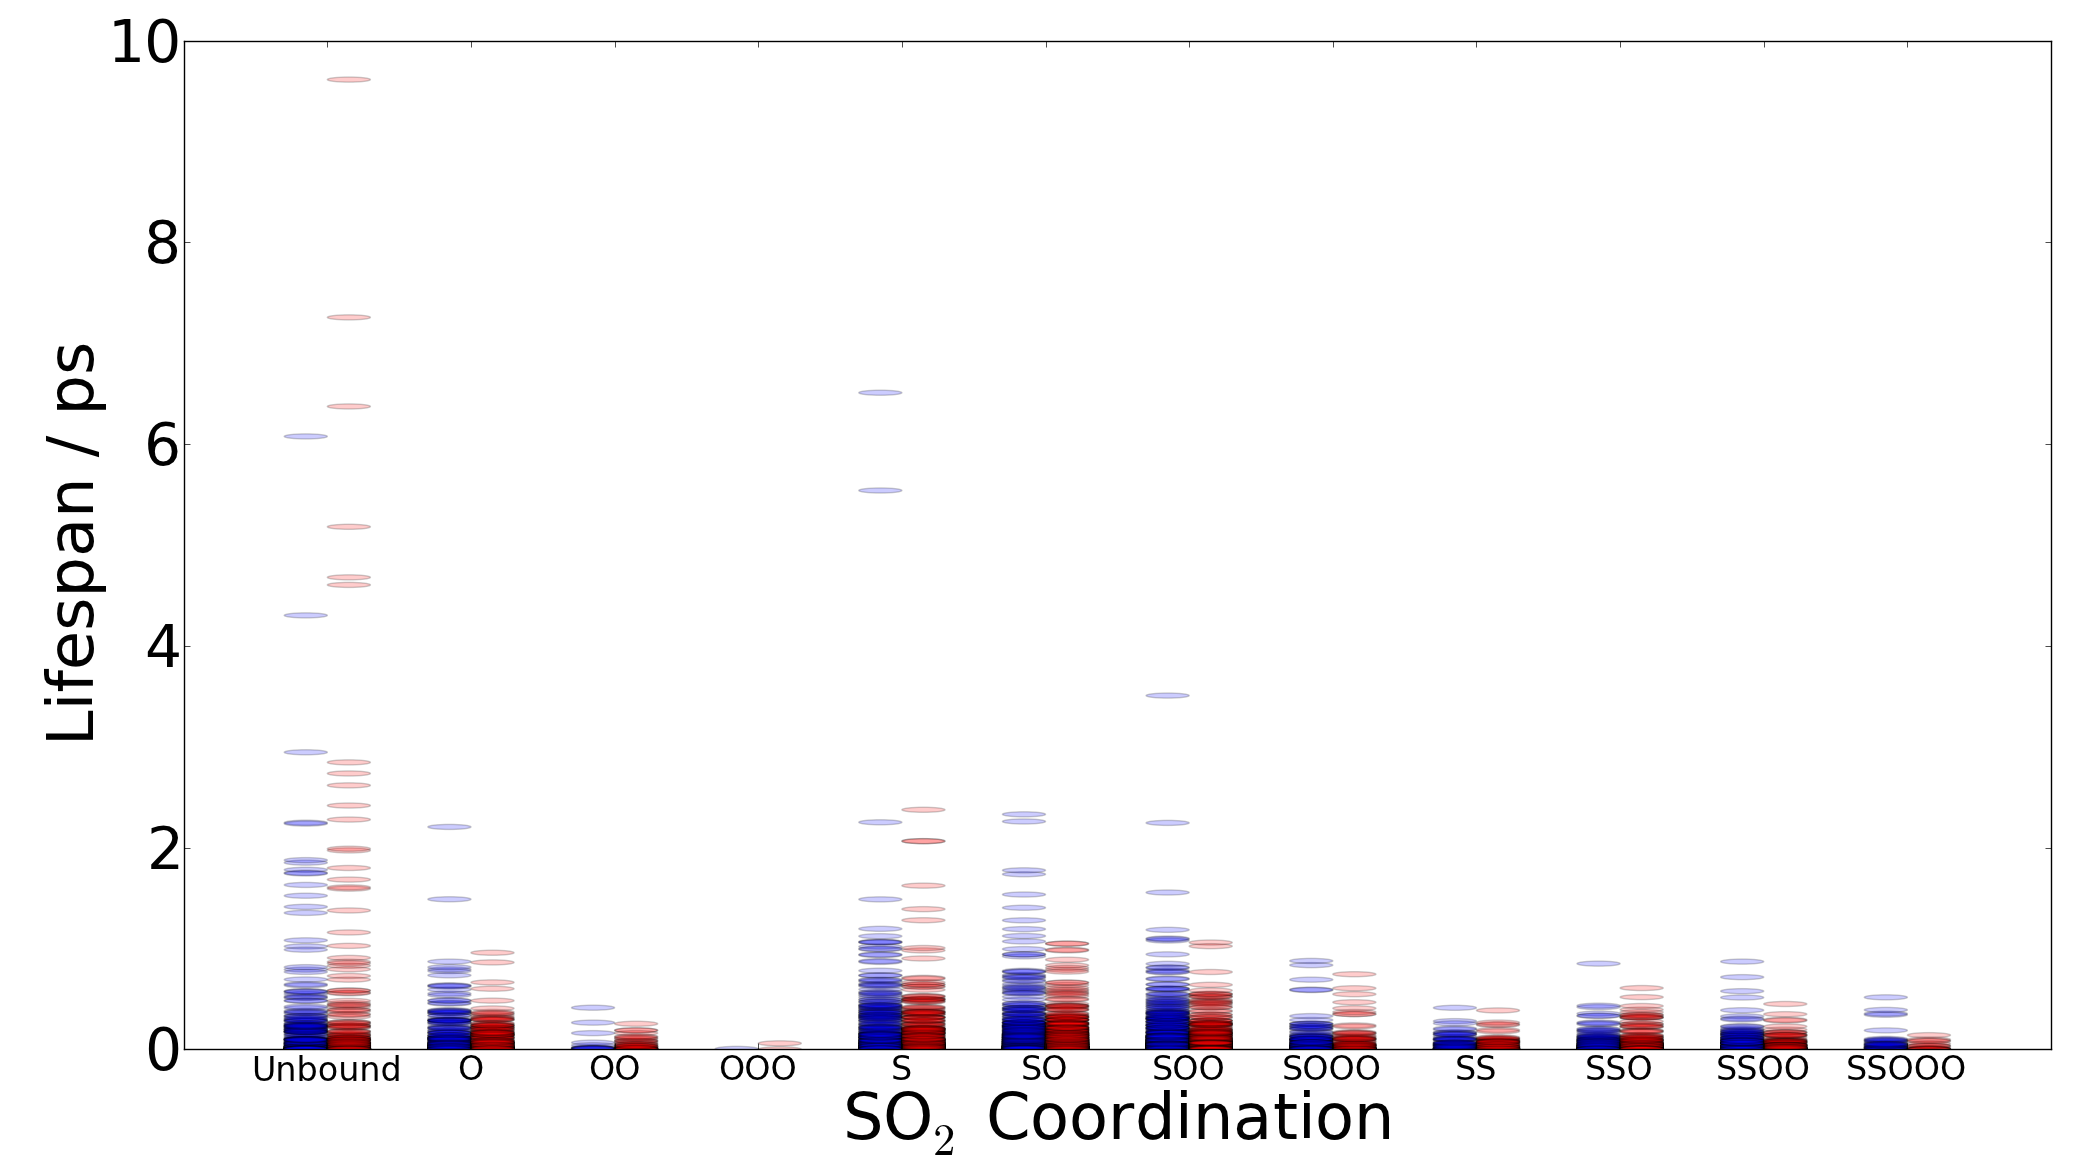
\includegraphics[scale=1.0]{coordination-lifespans.png}
		\caption{Given that certain bonding coordinations of the surface \suldiox~are more often encountered than others (see Figure \ref{fig:bonding-coordinations}), the plot here shows the time spent in each bonding coordination. Each point in the plot represents a single span of simulation time that the \suldiox~had the given coordination. The total amount of consecutive timesteps in a coordination corresponds to the vertical position along the lifespan axis, in ps.}
		\label{fig:coordination-lifespans}
	\end{center}
\end{figure}

Returning to the transition plots of Figure \ref{fig:coordination-transitions}, the behavior of the unbound transition to both ``S'' and ``O'' coordination can now be better characterized. Figure \ref{fig:coordination-lifespans} shows that the ``O'' coordinated lifetimes are slightly shorter than the ``S'' coordinated ones. Figure \ref{fig:coordination-transitions} shows that the unbound-``O'' transition occurs almost three times more than the transition to the ``S'' bonding coordination. The unbound \suldiox~forms a bond to a neighboring water through its oxygen, but that bond is short-lived and either quickly breaks (resulting in unbound \suldiox), or it transitions to the ``SO'' coordination by forming another bond through the sulfur. The unbound-``S'' transition does not occur as often. This may be because the ``S'' coordination is more stable than the ``O''. Once in the ``S'' coordination the \suldiox~does not quickly break the interaction from its sulfur to water, but rather remains for up to 2 ps in the ``S'' coordination before (most likely) forming an oxygen bond to make the ``SO'' coordination. We have outlined the likely behavior of \suldiox~as it transitions from the gas phase in an unbound coordination to binding to an aqueous interface by forming bonds and interactions with surface waters.

Once the \suldiox~begins interacting with the water surface, the pathway leading back to the unbound coordination is not often traversed. As shown in Figure \ref{fig:coordination-transitions} the dominant coordination transitions occur between the ``S-SO-SOO'' group of coordinations. This suggests that the \suldiox-sulfur interaction to a water oxygen has a much longer lifespan than the \suldiox-oxygen bonding to water hydrogens. The difference between the ``S-SO-SOO'' coordinations is an addition or removal of oxygen bonds. The frequent transitions between them show that the bonds to \suldiox-oxygens are quickly forming and breaking. For the \suldiox-sulfur interaction to break, the \suldiox~must enter a non-sulfur coordination (e.g. ``O'', ``OO'', unbound, etc.) or a coordination with more than a single sulfur interaction (e.g. ``SS'', ``SSO'', etc.). The transitions to coordinations that allow for breaking of the \suldiox-sulfur interactions, or switching the interaction to another water, are infrequent compared to those leading to an oxygen bond transition. Thus, the \suldiox~spends most of its time while bound to the surface waters breaking and forming hydrogen-bonds through its oxygens, and interacting with neighboring waters through a more persistent interaction via the \suldiox-sulfur atom.



% cycle results
\section {Cyclic \suldiox~Hydrate Structures}

Having examined the bonding coordinations and bonding behavior of \suldiox~with surface waters, we now turn to a secondary behavior of the hydrate structures that form around the surface-bound \suldiox~molecule. The simulation trajectory data was analyzed to determine the presence and characteristics of \suldiox~cyclic hydrate structures that form, as posited earlier in the text and depicted in Figure \ref{fig:cyclic-structures}. Only the most commonly occurring subset of the cyclic structures were analyzed based on two selection criteria: (1) The distances between atoms must match the same bonding/distance criteria as used for determining bonding coordinations. (2) The \suldiox~must be minimally in a bonding coordination of type ``SO'', meaning that the sulfur has at least one bonding interaction, and at least one hydrogen-bond must have formed with an oxygen to a neighboring water-hydrogen. As noted earlier in the discussion of the graph BFS algorithm, the cyclic structures found represent the smallest cycles in which the \suldiox~is a member, based on the search's order of cycle discovery. The \suldiox~will be involved in other larger and more extended cyclic bonding structures beyond the first one discovered via the BFS. The larger and more extended cyclic structures involving more waters affect the behavior of the hydrogen-bonding network of the water surface. We focus here only on the smallest cycles involving the \suldiox~as they most affect the \suldiox~bonding and hydration.

\begin{figure}[h!]
	\begin{center}
		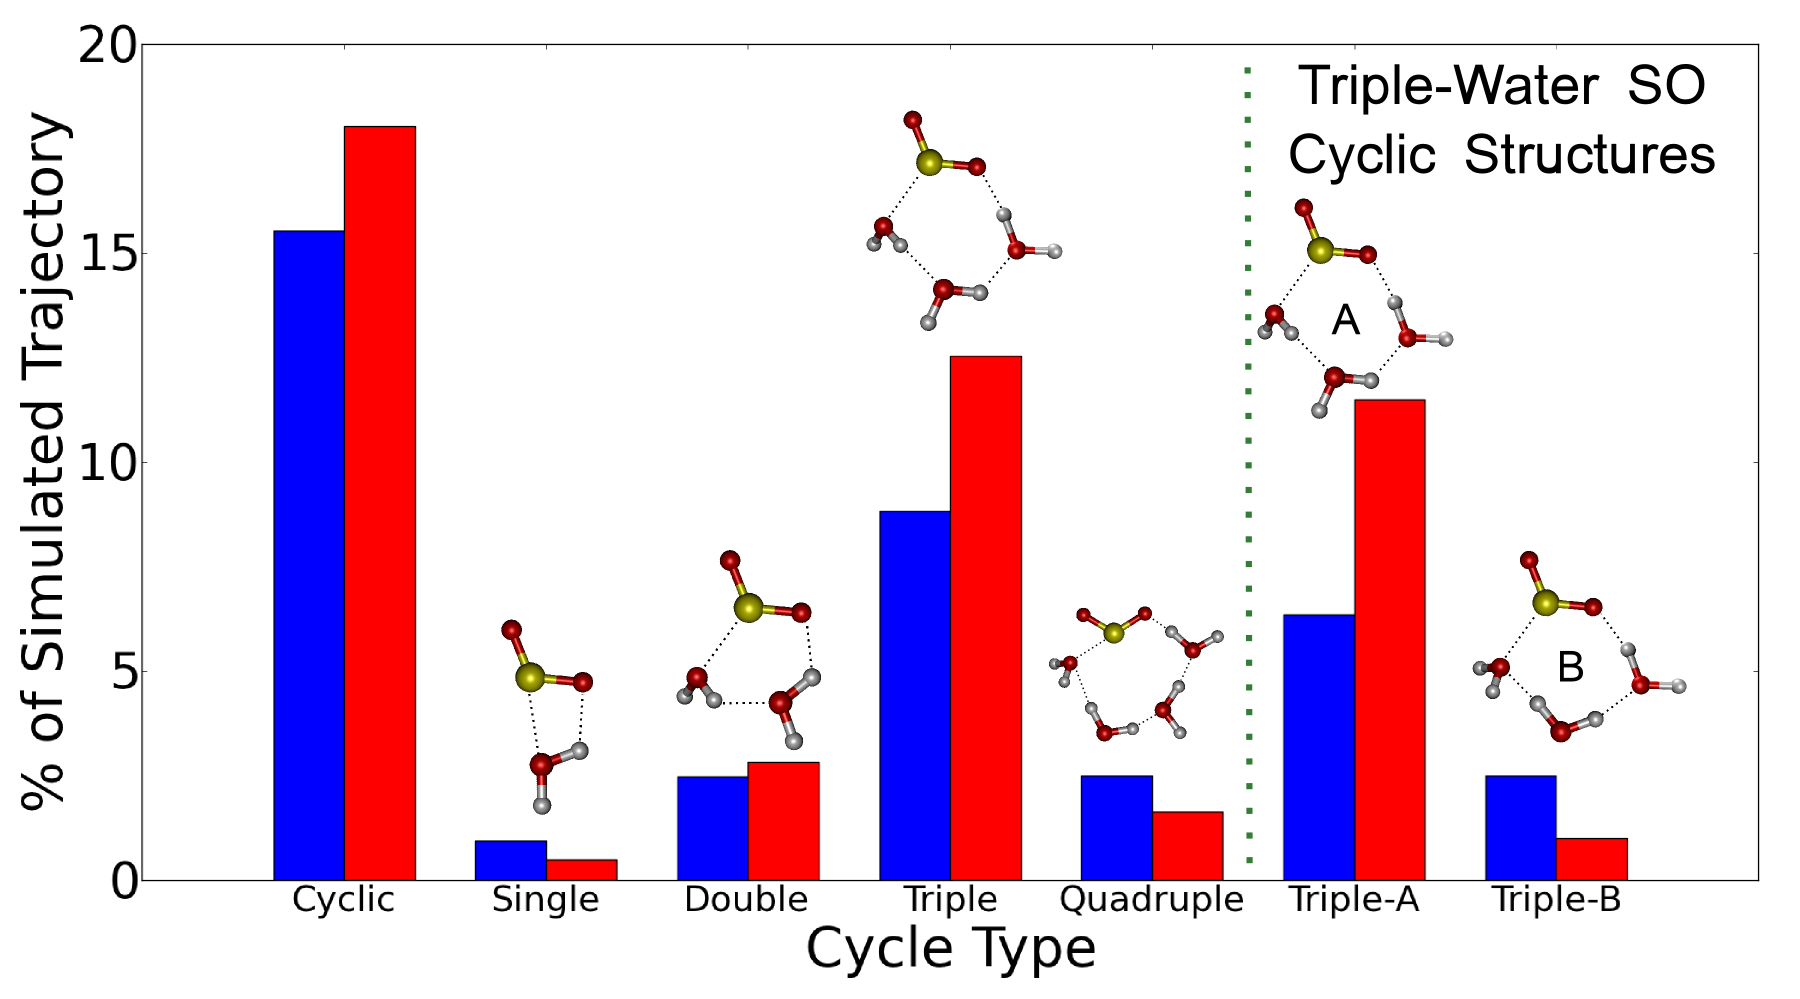
\includegraphics[scale=1.0]{cycle-distributions.png}
		\caption{Cyclic hydrate structures form throughout the MD simulations involving the \suldiox~and one or more water molecules. Shown here are the different cycles by number of water (up to 4), and their occurrence rate as a percentage of the total simulation time. The far right part of the plot shows the contributions of the two types of triple-water cycles (see Figure \ref{fig:type-3-varieties}). The cycles had to meet the ``minimally-SO'' bonding criteria (at least one bond to the sulfur and one oxygen bond on the \suldiox) to be used in the analysis.}
		\label{fig:cyclic-breakdown}
	\end{center}
\end{figure}

The plot in Figure \ref{fig:cyclic-breakdown} shows the distribution of how often the various types of cyclic hydrates were encountered at both cold (blue) and hot (red) temperatures. Each data point shows a percentage of the MD trajectories in which the \suldiox~was a member of a cyclic structure, for different numbers of cyclic waters (up to 4, ``Quadruple''). The two tallest data points labelled ``Cyclic'', left-most in the plot, show the overall time spent in all types of cyclic structures. Clearly the hot \suldiox~spends more time in a cyclic structure than at the cold temperature. The time spent in a cyclic structure shows a 2.5\% difference (15.5\% cold, 18.0\% hot) between the temperatures. Thus, in addition to having earlier found the most likely bonding coordination during the simulated life of \suldiox, we have also found that the hydrates of the \suldiox~form cyclic structures for much of the time while bound to the water surface.

Now we look at the different types of cyclic hydrates, distinguished by the number of waters involved in the bonding structure. In Figure \ref{fig:cyclic-breakdown} the single water cycles are the least frequently encountered structures, accounting for less than 1\% of both cold and hot temperature simulation times. Formation of the single-water type is likely energetically unfavorable because of the proximity of the water to the \suldiox~required to form the bonding cycle. The double-water structure was one of two types of clusters proposed in a previous computational work as a candidate structure contributing to the overall IR spectrum of surface-bound \suldiox.\cite{Baer2010} In those static and geometry-optimized cluster calculations, lacking the extended water structure or bonding from waters external to the hydrate, both the double and triple types appear equally likely to form. However, the MD simulations here have introduced many waters into a dynamic environment allowing for extended bonding networks, and the results show clearly that the double-water cyclic hydrate is formed much less often (less than 3\% at both temperatures) than the triple-water form.

The quadruple cycle types are similar in nature to the double type cycles. Likely the quadruple water cycles are not as favorable as the triple type because the size and number of bonds involved increases the possibility that some part of the cycle will break as another forms. Coordinating four waters to meet the cyclic hydrate criteria define here is likely what keeps the four-water cycles from forming often. The higher number of hydrating waters ($>$ 4) are not shown as those contribute minimally to the overall distribution. The majority of the cyclic hydrates are formed with three waters in the triple-water type. This hydrate type matches the bonding structure inferred from our previous experiments, and also one of the cluster types modelled by others.\cite{Tarbuck2005,Tarbuck2006,Baer2010} It was further found that, of the triple-type hydrate cycles, the waters contributing to the cycles can be arranged in two ways that preserve the hydrogen-bonding between the molecules (described earlier and shown in Figure \ref{fig:type-3-varieties}). The triple-water type cycle results were broken-down into contributions from the type-A and type-B triple-water structures. The two triple cycle structures are depicted on the right side of Figure \ref{fig:cyclic-breakdown}, along with the plots of their contributions to the overall distribution. It is notable that at both temperatures the dominant type of triple-water cyclic structure is in the ``Triple-A'' form. This form of the triple cycle corresponds to the resulting geometry from the calculations of Baer et al. and involved an equal contribution from each water in the cycle.\cite{Baer2010}

\subsection {Cyclic Hydrate Structure Lifetimes}

We know that the \suldiox~bound to a water surface is most likely in the ``SO'' bonding coordination, and is also often taking part in some type of cyclic structure. With this in mind, it becomes interesting to ask: how long does a cyclic hydrate form before breaking to an acyclic hydrate structure? To answer the question of cyclic lifespan, a method was devised to define the lifetime of a cycle. For each MD trajectory, coordinate data was analyzed to determine if a cyclic hydrate structure was formed as described earlier in this manuscript, and the lifespan data was collected as was done for the bonding coordinations. %A timeline was then produced where each timestep was given a value of 1 or 0 depending on whether a \suldiox~hydrate bonding cycle was present or not, respectively. This resulted in a time-function, $C(t)$, similar in nature to a time-varying digital signal. 

%In an electro-mechanical system, a mechanical switch often outputs a noisy signal, full of transients or ``signal bounce'' before settling to a final value. This will appear as a rapid on-off cycling of the signal, and the problem is one of great concern in signal processing. Many mechanical, electrical, and software solutions have been devised to suppress the transients, or ``debounce'' the signal. Analogously, the hydrate bonding cycles formed in the simulated system often undergo a period of time during formation, or before dissolution, where the $C(t)$ function bounces before settling into a final value. The bounce in the function manifests itself in our statistics as a series of rapid switches between cycle presence and cycle absence. Physically, the bond lengths within the cycle (or the cycle-to-be) are fluctuating back and forth across our bond-length criteria. It is thus an artifact of our algorithmic determination of the presence or absence of a bond. Removing this artifact will allow us to examine the longer-time bonding behavior and this is accomplished as follows. 

%We wish to find a function based on $C(t)$ that eliminates the brief oscillations during transitions. The resulting function, $f(t)$, will only contain information of whether a hydrate bonding cycle is present or absent, and none of the noisy oscillations of the transitions between the two states. $f(t)$ may then be used to calculate statistics about the cycle lifespans. A representative portion of a cycle time-function, $C(t)$, is plotted for one of the simulated trajectories shown as the dashed black line in Figure \ref{fig:debouncing}. At the far left of the plot the function is in the ``no cycle'' state indicating that a bonding cycle has not been detected, and then switches ``on'' as a cycle is found later in time. The cyclic structure is very dynamic, constantly moving and distorting, so any of the bonds forming the cyclic bonding structure are liable to break and reform quickly. This bouncing between states is manifested in Figure \ref{fig:debouncing} as a series of sharp spikes in the $C(t)$ function lasting less than 10 fs each. $C(t)$ was smoothed using a moving gaussian window function with a 10 fs width, having the effect of disregarding cycle breaks or formations of less than 20 fs duration. The resulting smoothed function, $C_s(t)$, was then cutoff with the following criteria:

%\[
%  f(t) = \left\{ 
%  \begin{array}{l l}
%    0 & \quad C_s(t) < 0.2\\
%    1 & \quad C_s(t) \geq 0.2\\
%  \end{array} \right.
%\]

%where $f(t)$ is the debounced time-function that represents the lifespans of cycles. Figure \ref{fig:debouncing} shows the original time-function of cycle formation and breaking, $C(t)$ (dashed black), the smoothed function, $C_s(t)$ (red), and the final debounced function, $f(t)$ (green).

%\begin{figure}[h!]
%	\begin{center}
%		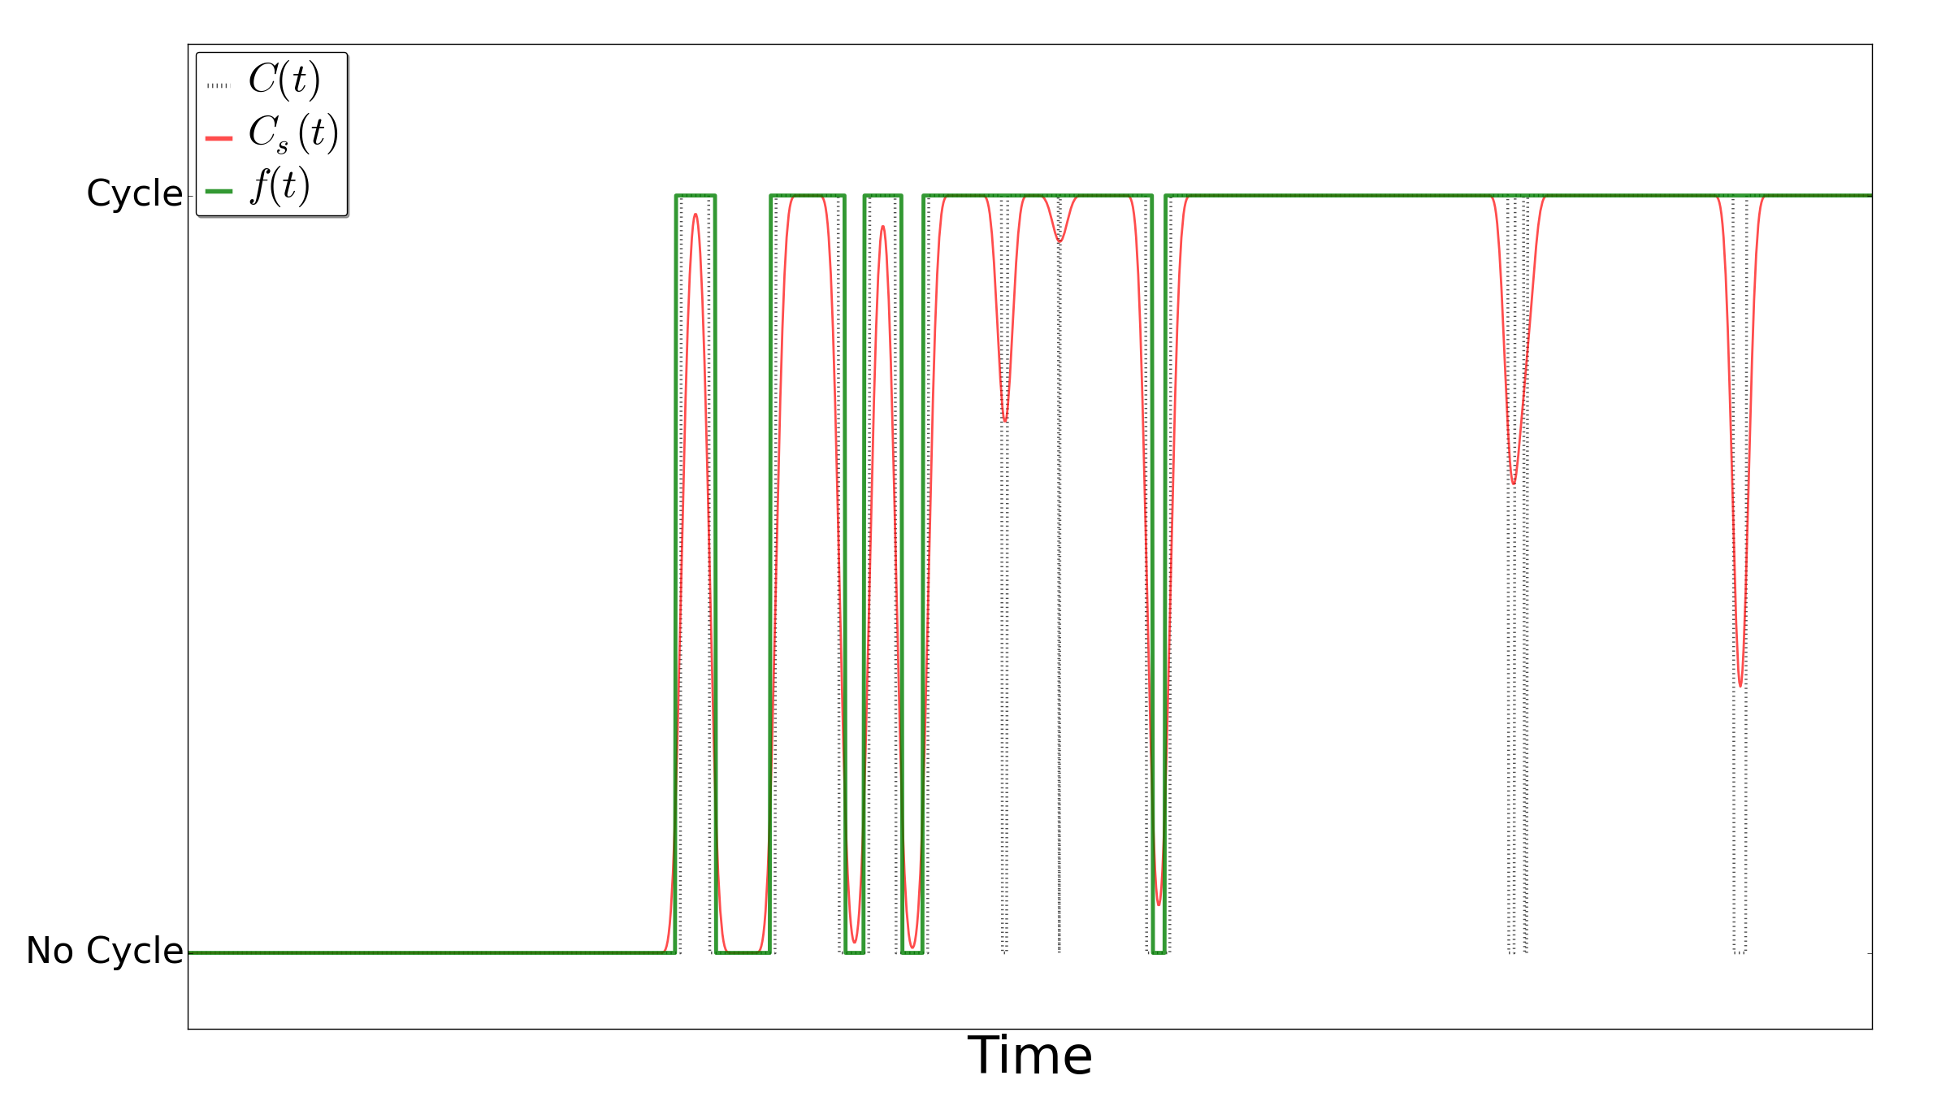
\includegraphics[scale=1.0]{cycle-debouncing-small.png}
%		\caption{The dynamic environment of the water surface causes rapid breaking and formation of bonds to the \suldiox, and to waters involved in the cyclic hydrating structures. A debouncing procedure was developed (described in the text) to account for the very brief ($<$ 20 fs) breaks to the cyclic structure. A time function, $C(t)$ (dashed black), shows if the bonding distance criteria are met for all members of the cyclic hydrate structure. A gaussian smoothing window was then used to produce $C_s(t)$ (red), which was then used with a cutoff criteria to give the debounced cycle formation time function, $f(t)$ (green).}
%		\label{fig:debouncing}
%	\end{center}
%\end{figure}

The distribution of cycle lifetimes (i.e. contiguous spans of time spent with a fully formed cyclic hydrate) was determined. The lifespans are shown in Figure \ref{fig:cycle-lifespans} for the cold (blue) and hot (red) simulations. The most frequent lifespan for both temperature data sets is less than 50 fs. This accounts for the vast majority of cyclic hydrates found (approximately 80\%) indicating that these structures are very transient, and are continuously forming and breaking for very short periods of time. The nature of the water surface, and the very dynamic extended hydrogen bonding network, keeps many of the structures from lasting much longer than a few fs. There is little difference between hot and cold systems in the $<50$ fs population, with this trend extending to the longer lifespans as well. The inset of figure \ref{fig:cycle-lifespans} shows an expanded view of the region above 0.2 ps. All of the distribution shows only a $<5$\% difference between cold and hot cyclic lifetimes. Overall, the distribution shows that when cycles form, at both temperatures, they last a similar amount of time. The cold system has more cycles forming than the hot system at the shortest cycle lifetimes ($<10$ fs). Up to 100 fs, the hot temperature cycles show a very slight population increase above the cold temperature cycles.

\begin{figure}[h!]
	\begin{center}
		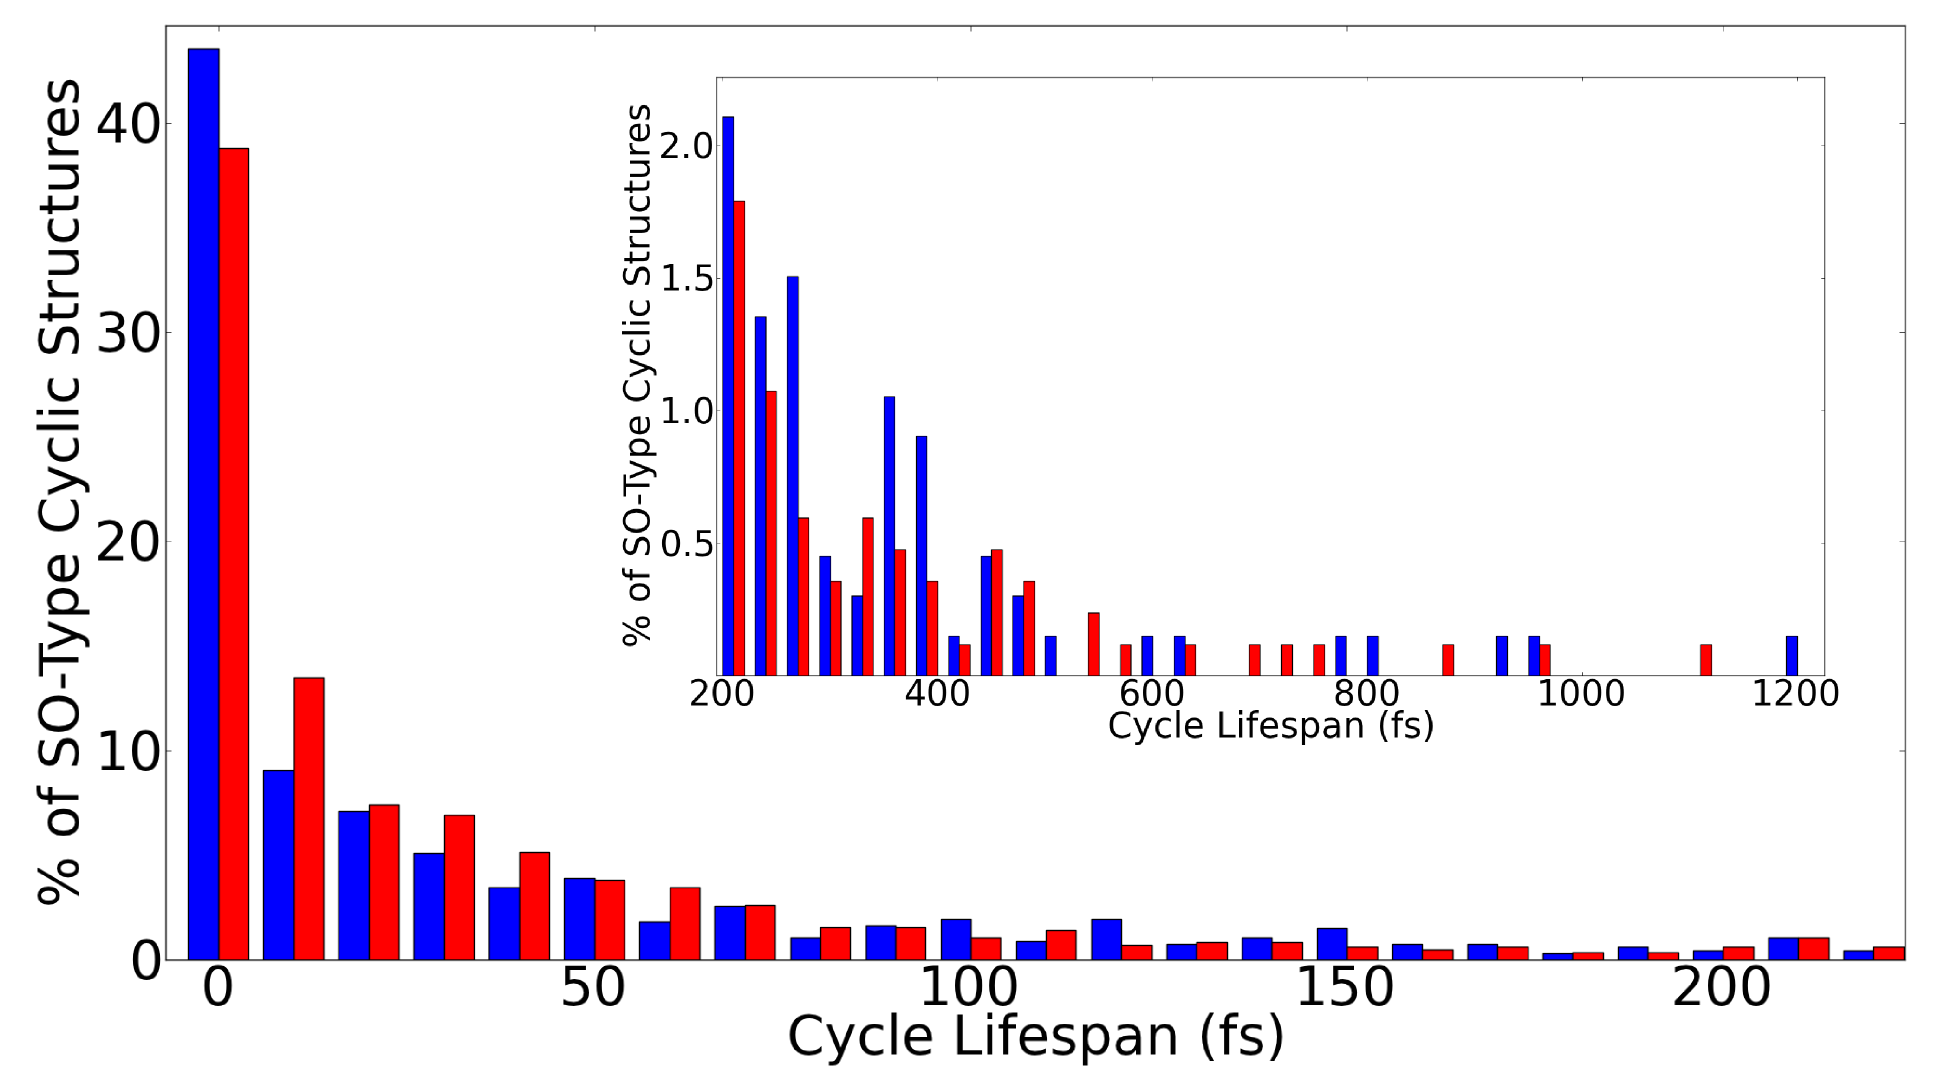
\includegraphics[scale=1.0]{cycle-lifespans.png}
		\caption{The lifetime of a cyclic hydrate structure after it forms, and before it distorts in shape due to the movement of the liquid surface molecules, is most often short ($<$ 50 fs). Shown here is a plot of cycle hydrate structure lifetimes. Both cold (blue) and hot (red) simulations are graphed. The inset expands the view of the region above 200 fs.}
		\label{fig:cycle-lifespans}
	\end{center}
\end{figure}

We know from the transition frequency plots of Figure \ref{fig:coordination-transitions} that the bonding coordinations are switching frequently. The \suldiox~is likely forming and breaking bonds with waters external to the cyclic hydrate structures (i.e. not directly involved in the bonds of the cycle). For the longer-lived cycles, the external bonding to the \suldiox~may have little effect on the cyclic hydrate waters. However, any time the \suldiox~switches into an unbound, sulfur-only, or oxygen-only coordination (i.e. ``S'', ``SS'', ``O'', etc), the cyclic structure is necessarily broken. Because the majority of cyclic structures last only briefly ($<1$ ps), the active switching of \suldiox~bonding coordinations appears to break the cyclic structure. Figure \ref{fig:bonding-coordinations} shows that the sum of coordinations that necessarily break cyclic structures account for approximately 51\% and 67\% of the bonding coordinations in the cold and hot system, respectively. Consequently, the distribution of Figure \ref{fig:cyclic-breakdown} also indicates that there are more cycles formed in the hot system (nearly 2.5\% above the cold). Of the most encountered bonding coordinations the hot system has a much higher proportion of unbound coordinations, and a relative decrease of the ``SOO'' coordination. The increased temperature appears to cause the \suldiox~to bond in a way that is slightly more conducive to the formation of cyclic structures. %This may account for the slightly increased populations of the longer cycle lifespans in the hot system (greater than 4 ps in some cases) compared to the cold system in the cycle lifespan distribution of Figure \ref{fig:cycle-lifespans}. 



%conclusions
\section {Conclusions}

The adsorption of small gas molecules to water surfaces has been extensively studied over the past few decades. Much has been learned about the energies of hydrate configurations, and the kinetics of gaseous uptake into aqueous systems. Yet, the specific molecular nature of the adsorption process, including the various geometries, hydrate species, and bonding pathways remains largely unknown. As a gas transitions into the liquid water phase, it passes through a fluid interfacial region that remains poorly understood. Our understanding of the processes and chemistry of the interface is still in its infancy, but we are beginning to gain unique new insights that are key to understanding many environmentally important processes at aqueous surfaces.

Presented herein are the results of ab initio molecular dynamics simulations that focus on how a wandering gaseous \suldiox~molecule first makes contact with a water surface, and subsequently forms extended hydrate structures with interfacial water molecules. The computational studies complement and expand on experimental studies from this laboratory that found surface complexation of \suldiox~at a water surface.\cite{Tarbuck2005,Tarbuck2006,Ota2011} Furthermore, these computations build upon and enrich our understanding of adsorbing \suldiox~behavior from our recently published computational study on interfacial geometries of aqueous surface \suldiox~molecules.\cite{Shamay2011}

Our simulations show that \suldiox~has a preferred means of bonding and interacting with surface water molecules by taking on various bonding coordinations. In this work it was shown that the ``SO'' bonding configuration is the most preferred, with ``S'' and ``SOO'' also contributing greatly to the coordination distribution. Once a \suldiox~has bound to form a surface hydrate it rarely forms multiple bonding interactions through the sulfur atom, and even less frequently takes on a configuration with no sulfur interactions to nearby waters.

This is one of very few temperature studies looking at the nature of microscopic behaviors of interfacial gas molecules on water. By changing the temperature, it was found that a colder water system leads to greater \suldiox~binding to the water surface. The distribution of bonding coordinations was greatly affected by a temperature change, shifting populations of bonding configurations because of the altered \suldiox~and \wat~behavior. At the lower temperature, \suldiox~forms more frequent bonds to interfacial waters through the sulfur and oxygen atoms. Overall, we have determined that the \suldiox~hydrate interactions are transient, binding and unbinding to water molecules rapidly in very dynamic bonding coordinations.

In this work we introduce the use of a graph structure to represent atoms and interconnectedness between molecules, and also to represent transitions between the various bonding coordinations of an adsorbed \suldiox. It was shown that the intermolecular bonds formed through the \suldiox-oxygens are quickly broken and formed, lasting briefly compared to sulfur interactions. From the graph of bonding coordination transitions, we found a likely pathway for \suldiox adsorption starting with an unbound gas-phase \suldiox, ending with a hydrated \suldiox~species bound to surface waters.

The formation of cyclic hydrate structures was probed and it was found that these hydrated bonding ring species form during much of a simulated trajectory. Higher temperatures slightly increase the occurrence of cyclic structures, and also shift the distribution of the specific types of cycles being formed. Two types of cyclic tri-hydrates were discovered during the course of simulations. The cycle lifetimes were found to be mostly short-lived, with a majority lasting only less than 50 fs before breaking and reforming due to the dynamic bonding and motion of the surface waters and \suldiox~molecules. Temperature did not have a very dramatic effect on the cyclic lifespans, but lower temperatures did lead to \suldiox~bonding coordinations that are more likely to form into cyclic hydrates.

These studies build upon our computational and experimental research in this area, seeking to understand how gases adsorb and transit across an aqueous/air interface. Such knowledge is invaluable for understanding land water and environmental aerosol systems where gaseous uptake behavior at a water surface surprises us and often defies our physical intuitions.\cite{Jayne1990,Yang2002,Worsnop1989,Boniface2000}


\section {Acknowledgements}

The authors would like to thank Dr. Daniel Steck of the University of Oregon Department of Physics for the generous use of computing resources, Dr. Kevin E. Johnson (Pacific University) and Dr. Fred Moore (Whitman College) for many informative discussions and insights, the National Science Foundation (Grant CHE-1051215), and the US Department of Education Graduate Assistance in Areas of National Need (GAANN) program (Grant P200A070436) for support of this research.

\bibliography{so2temperature}

\end{document}
